\documentclass[12pt]{article}  
%\documentclass[10 points,twocolumn]{article}
\usepackage{etex}
\usepackage{algorithm}% http://ctan.org/pkg/algorithms
\usepackage{algpseudocode}% http://ctan.org/pkg/algorithmicx
\usepackage{mathtools} % Bonus
\usepackage{hhline}
\usepackage{tikz}
\usetikzlibrary{trees}
\usetikzlibrary{shapes,arrows}
\usetikzlibrary{decorations.text}
\usepackage{tkz-graph}
% ========= UCF================================
\usepackage{graphicx}
\graphicspath{ {figures/} }
%==========Table ==============================
\usepackage{threeparttable}  
\usepackage{booktabs}
\usepackage{multirow}
\usepackage{bm}
\usepackage{float}
\usepackage{booktabs}
\usepackage{graphicx}
\usepackage[font=small,skip=10pt]{caption} % caption font and distance
\usepackage{subcaption}
\usepackage{paralist}
\usepackage{array} 
\usepackage{algpseudocode}
\usepackage{amsmath}
\usepackage{caption}
\usepackage{url}
\usepackage{multicol}
\usepackage{helvet}
\usepackage{courier}
\usepackage{amsmath}
\usepackage{amssymb}
\usepackage{xcolor}
\usepackage{rotating}
\usepackage{framed}
%==========Enume ===============================
\usepackage{enumitem}
\setlist[itemize]{leftmargin=*}
%==========Plot ================================
\usepackage{varwidth}% http://ctan.org/pkg/varwidth for formula indent

\usetikzlibrary{shapes,arrows,automata,shadows}
\usetikzlibrary{shapes.multipart}
\usetikzlibrary{positioning}%,calc}
\usepackage{pgfplots}
\pgfdeclarelayer{background}
\pgfdeclarelayer{foreground}
\pgfsetlayers{background,main,foreground}
\pgfplotsset{width=7cm,compat=1.8}
\usetikzlibrary{patterns}
\usetikzlibrary{matrix,fit}
%===========Listing ============================
\usepackage{listings}
\lstdefinelanguage{json}{
    basicstyle=\small\sffamily,
    showstringspaces=false,
    breaklines=true,
    frame=lines,
    backgroundcolor=\color{background},
}
%===========non italic math ====================
%\usepackage[LGRgreek]{mathastext} 
%===============================================
\newtheorem{definition}{Definition}
\definecolor{background}{HTML}{EEEEEE} %{EEEEEE}
%============Draw document symbol]==============
\makeatletter
\pgfdeclareshape{document}{
\inheritsavedanchors[from=rectangle] % this is nearly a rectangle
\inheritanchorborder[from=rectangle]
\inheritanchor[from=rectangle]{center}
\inheritanchor[from=rectangle]{north}
\inheritanchor[from=rectangle]{south}
\inheritanchor[from=rectangle]{west}
\inheritanchor[from=rectangle]{east}
% ... and possibly more
\backgroundpath{% this is new
% store lower right \usepackage{float}
in xa/ya and upper right in xb/yb
\southwest \pgf@xa=\pgf@x \pgf@ya=\pgf@y
\northeast \pgf@xb=\pgf@x \pgf@yb=\pgf@y
% compute corner of ‘‘flipped page’’
\pgf@xc=\pgf@xb \advance\pgf@xc by-20pt % this should be a parameter
\pgf@yc=\pgf@yb \advance\pgf@yc by-20pt
% construct main path
\pgfpathmoveto{\pgfpoint{\pgf@xa}{\pgf@ya}}
\pgfpathlineto{\pgfpoint{\pgf@xa}{\pgf@yb}}
\pgfpathlineto{\pgfpoint{\pgf@xc}{\pgf@yb}}
\pgfpathlineto{\pgfpoint{\pgf@xb}{\pgf@yc}}
\pgfpathlineto{\pgfpoint{\pgf@xb}{\pgf@ya}}
\pgfpathclose
% add little corner
\pgfpathmoveto{\pgfpoint{\pgf@xc}{\pgf@yb}}
\pgfpathlineto{\pgfpoint{\pgf@xc}{\pgf@yc}}
\pgfpathlineto{\pgfpoint{\pgf@xb}{\pgf@yc}}
\pgfpathlineto{\pgfpoint{\pgf@xc}{\pgf@yc}}
}
}

%============Margin ==================================
\setlength{\oddsidemargin}{0.005in}
\setlength{\textwidth}{6.5in}
\setlength{\topmargin}{-0.8in}
\setlength{\textheight}{8.9in}
%=====================================================
\tikzset{
box1/.style={draw=black, thick, rectangle,rounded corners, minimum height=3cm, minimum width=3cm},
box2/.style={draw=black, thick, rectangle, minimum height=4.5cm, minimum width=4.5cm},
}
%============ Arrow decoration =======================
\usetikzlibrary{arrows, decorations.markings}
% for double arrows a la chef
% adapt line thickness and line width, if needed
%\tikzstyle{vecArrow} = [thick, decoration={markings,mark=at position
%   1 with {\arrow[semithick]{open triangle 60}}},
%   double distance=1.4pt, shorten >= 5.5pt,
%   preaction = {decorate},
%   postaction = {draw,line width=1.4pt, white,shorten >= 4.5pt}]
%\tikzstyle{innerWhite} = [semithick, white,line width=1.4pt, shorten >= 4.5pt]
%========================================================
%appendix
\usepackage[title,titletoc,toc]{appendix}

\renewcommand{\algorithmicensure}{\textbf{Output:}}



\usepackage{color}   %May be necessary if you want to color links
\usepackage{hyperref}
\hypersetup{
    colorlinks=true, %set true if you want colored links
    linktoc=all,     %set to all if you want both sections and subsections linked
    linkcolor=black,  %choose some color if you want links to stand out
	citecolor=black,
    urlcolor=blue,
}
%========================================



\begin{document}
% Draw background
\newcommand{\background}[5]{%
\begin{pgfonlayer}{background}
% Left-top corner of the background rectangle
\path (#1.west |- #2.north)+(-0.5,0.25) node (a1) {};
% Right-bottom corner of the background rectanle
\path (#3.east |- #4.south)+(+0.5,-0.25) node (a2) {};
% Draw the background
\path[fill=gray!20,rounded corners, draw=black!50, dashed]
(a1) rectangle (a2);
\path (#3.east |- #2.north)+(0,0.25)--(#1.west |- #2.north) node[midway] (#5-n) {};
\path (#3.east |- #2.south)+(0,-0.35)--(#1.west |- #2.south) node[midway] (#5-s) {};
\path (#3.east |- #2.north)+(0.7,0)--(#3.east |- #4.south) node[midway] (#5-w) {};
\end{pgfonlayer}}

\newcommand{\transreceptor}[3]{%
\path [linepart] (#1.east) -- node [above]
{\scriptsize #2} (#3);}

% Define block styles
\tikzstyle{startstop} = [rectangle, rounded corners, minimum width=3cm, minimum height=1cm,text centered, draw=black, fill=white]
\tikzstyle{process} = [rectangle, minimum width=3.0cm, minimum height=1cm, text centered, draw=black, fill=white]
\tikzstyle{decision} = [diamond, draw, fill=white, 
text width=4.5em, text badly centered, node distance=3cm, inner sep=0pt]
\tikzstyle{line} = [draw, -latex']
\tikzstyle{cloud} = [draw, ellipse,fill=red!20, node distance=3cm,minimum height=2em]
\tikzstyle{arrow} = [thick,->, >=stealth]    
\tikzstyle{io} = [trapezium, trapezium left angle=70, trapezium right angle=110, minimum width=3cm, minimum height=1cm, text centered, draw=black, fill=white]
%=============================================
% Defined for chart and background
\tikzstyle{square}=[rectangle,thick,minimum size=0.5cm,draw=blue!80,fill=blue!20]
\tikzstyle{vspecies}=[rectangle,thick, text centered, drop shadow, minimum size=0.5cm,draw=black,fill=white]
\tikzstyle{invspecies}=[rectangle,thick, text centered, minimum size=0.5cm,draw=black,fill=white]
\tikzstyle{square}=[rectangle,thick,minimum size=0.5cm,draw=red!80,fill=blue!20]
\tikzstyle{fspecies}=[rectangle, minimum size=0.5cm,draw=red!80,fill=red!20]
\tikzstyle{ur}=[draw, text centered, minimum height=0.01em]
\tikzstyle{linepart} = [draw, thick, color=black!50, -latex', dashed]
\tikzstyle{database}= [ cylinder, cylinder uses custom fill,cylinder body fill=white, cylinder end fill=white, shape border rotate=90,      aspect=0.20, draw]
%=====================================================
\title{On information leakage in cloud database services}
\author{Mohammad Ahmadian and Dan C. Marinescu \\
Department of Computer Science University of Central Florida,\\ Orlando, FL 32816, USA\\
Email: \{ahmadian, dcm\}@cs.ucf.edu}
\date{\today}
\maketitle

\tableofcontents

\section*{Abstract}
Web and mobile applications take advantage of the Database as a Service (DBaaS) to access the very large number of databases stored on computer clouds. The popularity of DBaaS amplifies the security risks for cloud stored data, even if encrypted, and exposes an information leakage channel that can be exploited by cross-referencing  cloud-hosted databases. Very large databases stored on computer clouds include data with various degrees of sensitivity. The sensitivity analysis discussed in this paper identifies the most valuable information that must be protected for limiting the effects of information leakage. The methods we propose are based  on the Approximate Query Processing (AQP) technique.  We report on experiments conducted to assess the effectiveness of AQP.
 
%\part{Leakage management}
%*************************************************
\section{Introduction and Motivation}
\label{sec:introduction}
%*************************************************

Information leakage is the inadvertent disclosure of sensitive information. Information leakage enables an attacker to infer sensitive information either through multiple database searches or through a statistical analysis of database queries.  The threat posed by information leakage is amplified  as cloud data warehouses maintain a large number of hosted databases from various organizations.   

Information linkablity, the ability to link individual items of information from different sources poses a new type of threat to cloud users��.  An attacker could link low-risk pieces of information to extract the sensitive information. For example, a metro card connected to user's debit card for auto-refill could allow a cross-correlation revealing  sensitive financial information. Moreover, personal information from the financial record could be linked to the health record of the individual. 
 
Nowadays, many enterprises use DBaaS offered by major Cloud Service Providers (CSPs) to access the increasingly larger  number of cloud hosted databases  \cite{cloudcomputing17}.  A $67\%$ annual growth rate is predicted for DBaaS by $2019$.  CSPs guarantee availability and scalability, but the data confidentiality poses significant challenges in the face of new threats. Some of the threats emanate from insider attackers who have the ability to correlate information from multiple cloud databases. 

Information leakage  from unencrypted, as well as  encrypted cloud databases is possible.  A database can be encrypted before being outsourced to the cloud, yet allow  client queries to be processed on the transformed data. Data encryption provides data and query privacy but, contrary to the common belief, encrypted cloud data and encrypted queries are vulnerable to information leakage. The leakage can be exploited by external, as well as insider agents. 


Encryption does not hide all information about the encrypted data. A malicious insider can infer sensitive information through cross-referencing with other databases in the data warehouse. Moreover, the collection name, the attribute name (or table, field name in RDBMS), the number of attributes involved in a query, and the query length often reveal sensitive information about the encrypted data. 

A motivating sequence of events illustrate the effects of data correlation and, implicitly of information  leakage. In August 2006, AOL, a global on-line mass media corporation,  released search logs of over 650\,000 users for research purposes. The data included searches conducted over a period of three months with user names changed to random ID numbers. An analysis of the searches conducted by a user, made him/her uniquely identifiable. Correlating data released by AOL with publicly available datasets revealed additional private information about AOL users.

The discussion in this paper is restricted to  NoSQL databases with a flexible schema. A NoSQL database is a collection of documents $D={d_1,\dots,d_n}$. A document is a set of key-value pairs ${key_i, value_i}$, each representing an attribute of an object. Enforcing partial security mechanism which covers only a subset of attributes, may not provide comprehensive protection as protected information could be inferred using low-risk datasets hosted by the same cloud. 


A procedure to search an encrypted datasets involving a secure proxy, the \emph{ SecureNoSQL} \cite{Ahmadian2016SecureNoSQL} guarantees that an insider attacker would never obtain the decryption keys. The proxy encrypts the queries from the clients and decrypts the query responses from the server. The process is completely transparent, without the clients being involved in encryption/decryption operation. The proxy construction assures that an insider attacker could not access to the sensitive information. However, the insider attacker can exploit leaked information from multiple databases to organize more extensive attacks and amplify leakage.

The number of documents in  cloud databases  limits the  ability to analyze in real-time the dangers posed by information leakage. The alternative we  propose is based on random sampling and error estimation regarding information leakage. This  solution dramatically cuts the analysis time, especially, whenever the sample size is small enough to fit in the main memory of the database servers.  As expected, approximate measurements based on data sampling  exhibit different levels of errors. Sampling-based Approximate Query Processing (AQP) provides bounds on the error caused by sampling \cite{agarwal2014knowing, chatzikokolakis2009calculating}.


We propose insertion of \emph{disinformation documents} into the collection. A  secure proxy like the one in \cite{Ahmadian2016SecureNoSQL} mediates the interaction between clients and the DBaaS server. The proxy intercepts the client queries, transfers them to the encrypted queries and passes them to the cloud DBaaS server which responds with a combination of valid and forged documents. 

Eventually, the proxy decrypts the query response and filters out the fake documents and forwards the desired document to the user's application.  The Selective Disinformation Document Padding (SDDP)  is proposed  to avoid the overhead of disinformation document padding in the dataset.   We also investigate an Encrypted Data Indexing features for minimizing the query processing time of augmented ciphertext datasets. The contributions of this paper are:

\begin{enumerate}[leftmargin=*]
\item 
A method to quantify exact volume of information leakage as a result of explicit and implicit attribute cross-correlations in a cloud data warehouse.
\item
A selective disinformation document padding method to reduce information leakage with limited overhead.
\item 
A scalable leakage assessment and parameter extraction algorithm for very large databases based on approximate query processing.
\end{enumerate}
%****************************************************************************
\section{Security schemes for cloud database services}
\label{sec:relatedWork}
%*****************************************************************************

Query processing for outsourced databases is reported in  \cite{popa2011cryptdb,Ahmadian2016SecureNoSQL,7889242}. A common practice is to apply a cryptosystem  before releasing a database to a service provider and to  encrypt the queries as well. For instance, CryptDB \cite{popa2011cryptdb} can be used for encrypted SQL-based cloud databases, while SecureNoSQL  \cite{Ahmadian2016SecureNoSQL} for encrypted NoSQL databases. 

These two systems do require modifications of database services, encrypted data is processed identically as the plaintext data. Database optimizations such as multi-layer indexing and cache and file management are applied to encrypted databases without any modifications. However, neither of existing systems address information leakage of encrypted data.

Full Homomorphic Encryption (FHE)  allows computations to be performed on ciphertext. Decryption of the results of these operations are identical with the results of operations performed on the corresponding plaintext.  HE is theoretically feasible \cite{gentry2010computing}, but impractical due to the enormous overhead involved.

Order Preserving Encryption (OPE) scheme is a deterministic cryptosystem where encryption of numeric data preserves the ordering of the plaintext data. Aggregate queries such as comparison, min, and max can be executed on OPE encrypted datasets. OPE offers less protection than FHE and leaks critical information about the plaintext data \cite{ahmadian2014security, boldyreva2009order}. 

Searchable encryption methods such as Oblivious RAM (ORAM) \cite{liu2014search, ostrovsky1990efficient} provide an acceptable level of security. However, the efficiency and the high computational cost, as well as the excessive communication costs between the clients and the server make this method impractical \cite{goldreich1996software}.

Inference attacks against CryptDB was first proposed in \cite{naveed2015inference}. A series of attacks to the encrypted databases were designed under CryptDB, especially those encrypted with property preserving crypto-systems. Deterministic and OPE cryptosystems leak  critical information such as frequency and order of the original data, and therefore enable the attackers to extract sensitive information. The literature on managing information leakage in the cloud shows a variety of approaches. Two major research approaches include (i) restriction on the sequence of queries or query processing time; and (ii) insertion of fake documents.

A quantitative characterization of correlation-based information leakage, formulated through the capacity of a $(n,q)-leakage$ channel is studied using restriction on the number of query or query processing time \cite{4221659}. The n-channel capacity is defined as the maximum possible depth of query-able information for any user. The capacity of a n-leakage channel, is defined as the probability of accessing a specific sensitive document in $n$ trials. In this approach, a group of documents form a chain with track of key-value pairs, and attacker can locate the head of the chain. By following the footprints, the rest of sensitive information can be accessed. The attacker is not only constrained by the number of trials, but also by the time necessary to achieve his objectives.

There are two major approaches to manage information leakage. The first approach is built upon the dependency graph of sensitive attributes scattered in the multiple collections stored in cloud warehouse. In fact, the query sequence is mapped on the dependency graph, and according to the defined policy, at some points, the queries should be prevented from execution. More specifically this method is about keeping track of queries and when the accumulated leaked information reaches to the maximum level of disclosure; the proxy prevents any more queries from being executed. This method is vulnerable when it is subjected to collaborative attacks, or in particular, when multiple users are trying to pass partial result to the next user to obtain the maximum leakage. Evidently, this method is not effective against MI \cite{4221659}.

To reduce the risks posed by information leakage second approach propose insertion of fake documents in the database.  The fake information is expected to mislead the attacker by providing multiple values to an attribute. This solution drastically increases the number of total documents, the search time, and the communication costs\cite{whang2010managing}. However, multi-level indexing could reduce the query processing time in this case.

The number of the database limits the  ability analyze the level of information leakage between data elements in real-time. Random sampling for approximate measurement dramatically cuts the analysis time, especially, whenever the sample size is small enough to fit in the main memory. of the database server However, approximate measurements based on sample data show different levels of inconsistency with measurements on the entire database. Sampling-based Approximate Query Processing (AQP) provides bounds on the error caused by sampling \cite{agarwal2014knowing, chatzikokolakis2009calculating}.

Assessing the leakage from large datasets is a kind of problem that can tolerate some degree of inaccuracy. Therefore, we adopt the same approach in this work. In this work, the multi-level indexing and sampling-based approximate query processing is used as our first approach to avoid high latency of query processing. The second approach introduced in this work is selective disinformation document insertion based on the statistical analytics of data. This solution reduces the size of the expanded dataset and decreases the  overhead, the computational cost, and the response latency. 

\medskip

Cloud data can be in three states store, transit, or process and any comprehensive data security mechanism must protect data in any of these three states. The communication channels can be secured using standard HTTP over the SSL (Secure Socket Layer) communication protocol. 

Most CSPs provide an API for the web service that enables developers to use both the standard HTTP and the secure version of the HTTPS protocol. The security requirements of data in transit state can be fully satisfied using HTTPS for communication with cloud. The endpoint authentication feature  SSL makes it possible to ensure that the clients are communicating with an authentic cloud server.

The basic idea is to encrypt the data before uploading it to CSP. However, the data should be decrypted by the cloud server before getting processed. In other words, the data owner should disclose decryption key to the server in order to decrypt the data before performing any required operation. The problem is when the decryption key is compromised, the data confidentiality would be affected. Therefore, in the cloud computing environment new cryptosystems are required. 

\medskip


\noindent \textbf{\textit{Random (RND):}} In  a RND type encryption scheme, a message is coupled with a key $k$ and a random Initial Vector (IV). This scheme is non-deterministic, encryption of the same message with the same key yields different ciphertext. This randomness provides the highest level of security. 

The randomness property is achievable with different encryption algorithms. Advanced Encryption Standard (AES) with Cipher Block Chaining (CBC) mode is used for RND encryption. AES is a symmetric block cipher algorithm with a key size of 128,192 or 256 bits and with a block size of 128 bits. RND type schemes are semantically secure against chosen plaintext attacks and hides all kinds of information about ciphertext. As a result, RND scheme does not allow any efficient computation on the ciphertext. Equation \ref{eq1} describes the encryption and decryption of a block cipher in CBC mode.

\begin{equation} 
\label{eq1}
\begin{aligned}
for \quad j=2 \ldots n ;\qquad  \begin{cases}
C_1  = E_k(P_1 \oplus IV), \qquad  P_1 &= IV \oplus D_k(C_1) \\
C_j  = E_k(P_j \oplus C_{j-1}), \quad 
P_j &= C_{j-1} \oplus 
D_k(C_j)\\ 
\end{cases}\\
\end{aligned}
\end{equation}

\medskip

\noindent \textbf{\textit{Deterministic (DET):}}  A DET encryption scheme produces the same ciphertext for an identical pair of plaintext and key. Block ciphers in Electronic Code Book (ECB) mode, with a constant initialization vector are deterministic (DET). Deterministic encryption scheme preserves equality, therefore, the frequencies information of the searched keywords leaks to the third party. 

AES scheme in ECB mode is used for DET encryption over document-oriented NoSQL databases. DET scheme enables server to process pipeline aggregation stages such as group, count, retrieving distinct values and equality match \footnote{Equality matches over specific common fields in an embedded document will select documents in the collection where the embedded document contains the specified fields with the specified values.} on the fields within an embedded document. The embedded document can maintain the link with the primary document through application of DET encryption. Equation \ref{eq2} describes the encryption and decryption operation in a DET.

\begin{equation} \label{eq2}
\begin{aligned}
for \quad j=1, \ldots, n ;  \qquad \qquad  C_j & = E_k(P_j); \qquad \quad 
& P_j & = D_k(C_j) 
\end{aligned}
\end{equation}
\normalsize Where: $E_k$ is the encryption algorithm, $D_k$ is the Decryption algorithm, $k$ is the secret key, $P$ is a block of plaintext data and $C$ is a block of ciphered data.


\normalsize

\medskip

\noindent \textbf{\textit{Order-Preserving Encryption (OPE):}} OPE projects the order relation between plaintext data elements and their ciphertext values. OPE leaks the order of ciphertext, so it supports a lower degree of security. Even in Modular Order-Preserving Encryption (MOPE) \cite{Mavroforakis:2015:MOE:2723372.2749455} which is an extension to the basic OPE for security improvement, there is information leakage. An efficient inequality comparisons on the encrypted data elements can be performed by applying OPE which supports range queries, comparison, min and max on the ciphertext. We use the algorithm introduced in \cite{boldyreva2009order} and implemented in \cite{ahmadian2014security} for cloud environment. Equation \ref{eq3} shows the preservation of order relation of plaintext in the ciphertext.

\begin{equation} \label{eq3}
\begin{aligned}
\forall x, ~y ~|~ x,~y~ \in {Data~ Domain} \qquad x < y  \implies  OPE_k(x) < OPE_k(y)
\end{aligned}
\end{equation}

\normalsize Where $OPE_k$ is key-based OPE.


\medskip 

\noindent \textbf{\textit{Additive Homomorphic Encryption (AHOM):}} AHOM allows the server to conduct computations on ciphertext with the final result that is decrypted at the proxy. In spite of sustained research efforts \cite{gentry2009fully, brakerski2014efficient} of the Fully Homomorphic Encryption (FHE), there is no efficient FHE, except for some limited operations. AHOM is formulated in Equation \ref{eq4}. It should be noted that  $m_1, m_2$ are messages to be encrypted where $m_1 , m_2 \in \mathbb Z_{n}$. $r_1, r_2$ are randomly selected and $r_1, r_2 \in \mathbb Z^{*}_{n}$. In other words, the product of two ciphertexts decrypt to the sum of their corresponding plaintexts.

\begin{equation} \label{eq4}
\begin{aligned}
D_k(E_k(m_1, r_1) \times E_k(m_2, r_2) ~mod ~n^2) & = m_1 + m_2~ (mod~ n) 
\end{aligned}
\end{equation}

In this paper whenever the summation and multiplication operations are carried out over encrypted data, we applied Paillier \cite{paillier1999public} scheme which is an instance of AHOM.

Data granularity indicates the level of detail, the more detail, the higher granularity level.
Encryption can be applied for datasets at various levels of granularity from high granularity data, like atomic level data element to low level granularity in aggregated atomic data items. For data store encryption, it is conceivable to have different encryption granularity levels according to the corresponding data granularity. 

The higher level of encryption granularity, the higher the information leakage. For example, encryption of a single attribute leaks frequency information, while encryption of the entire  document and collection as a single unit leaks less information. In the work reported in this paper  we use different encryption granularity matching the data granularity level. 


%*************************************************************
\section{System Models and Assumptions}
\label{sec:systemModel}
%*************************************************************
\noindent {\bf The threat model.} This study is focused on system end-to-end security based on an adversarial perspective.  Call  $W_{DBaaS}$ the set of databases managed by a DBaaS:

\begin{equation}
\label{eq:DBaaS}
W_{DBaaS}=\Big \langle D_1,\dots, D_n \Big \rangle
\end{equation}
Each database $D_{i} ~, ~~ 1 \le i \le n$ consists  of an arbitrary number  $m$ of documents:

\begin{equation}
\label{eq:Database}
D_\imath = \big\{ d_1,\dots,d_m\big\}\\
\end{equation}
A document $d_{j}~,~~1 \le  j \le m$ includes an arbitrary number $l$ of key-value pairs $\langle key, value\rangle$: 

\begin{equation}
\label{eq:Document}
d_\jmath=\big\{ A_1,\dots, A_l\big\} 
\end{equation}

\noindent The function, $\Psi_{\epsilon}(D_i,D_j)$ in Equation \ref{eq:attributeCorrelation} is used to measure the information leakage $\mathcal{L}$ from any given pair of two databases $D_P$ and $D_Q$ as a result of cross-correlation:   

\begin{equation}
\label{eq:attributeCorrelation}
\begin{aligned}
\Psi (D_P, D_Q):
& \forall~d_p \in D_P ~\land~ \forall~ d_q \in D_Q ~~if~~ (\mu(d_p,d_q)==True) \implies \mathcal{L}=\Delta(d_p, ~d_q) 
\end{aligned}
\end{equation}

Where $\mathcal{L}$ is set of the leaked attributes and the operator $\Delta$ is the symmetric difference operator which is the union of all attributes from both documents without the intersection, and '\textbackslash' ~ is relative complement. The $\Delta$ can be restated as $\Delta(d_p, ~d_q) =(d_p\setminus d_q)\cup (d_q\setminus d_p)$.

\noindent The feasibility function $\mu$ in Equation \ref{eq:attributeCorrelation} determines if a given pair of documents can be merged according the type of shared attribute. The $\mu$ function is outlined in Equation \ref{eq:muFunction}.


\begin{equation}
\label{eq:muFunction}
\begin{aligned}
& \mu(d_p,d_q)= \begin{cases}
&\textbf{True} \\
&iff \quad \exists A_r \in d_p ~ \land ~\exists A_s \in d_q ~ \mid [(A_r.key==A_s.key) \land (A_r.value==A_s.value)]\\
\noalign{\text{Such that $A_r, A_s$ are indentifier attributes of $d_p, d_p$}}
&\textbf{False} \qquad Otherwise
\end{cases}
\end{aligned}
\end{equation}

An adversarial threat analysis starts with thinking like an attacker and continues to prepare the corresponding countermeasure. Two classes of threats, external and internal attackers are identified by the model. External attacks can be conducted after obtaining unauthorized access to data or by using tools to monitor the communication between the clients and the cloud servers. External attackers face a more complex task since they need to bypass firewalls, intrusion detection systems, and other protection mechanisms.


Insider attacks can be conducted by the employees and the contractors of large data centers with access to the software, the hardware, and the data. A malicious insider could leak highly sensitive documents or use it for nefarious activities. There is also the risk of an intruder gaining the same level of access using the credentials of a legitimate employee. An insider can bypass internal protection mechanism and pose serious risks to data \textit{confidentiality}, \textit{integrity} and \textit{inference} violations. The list of possible insider attacker actions are denoted as $A=\{C, I,\Psi \}$ respectively.

The risk factors and the corresponding solutions as well as the advantages and disadvantages of the proposed solution are summarized in Figure\ref{fig:MIriskFactors}.

\begin{figure}[H]
\centering
\resizebox{0.9\textwidth}{!}{\begin{tikzpicture}[
block/.style={rectangle,draw,fill=gray!20,text width=9em,text centered,rounded corners,minimum height=4em,node distance=0.4cm,auto},
line/.style={draw,-latex',node distance= 2cm,auto}]

\node [block] (a) {Confidentiality violation};
\node [block, below=of a] (b) {Integrity violation};
\node [block, below=of b] (c) {Information leakage};

\node [block, right=of a] (sa) {Cryptosystems:\\AHOM, OPE, \\DET, RND };
\node [block, right=of b] (sb) { Query verification};
\node [block, right=of c] (sc) {1-Query tracking\\2-Selective insertion of disinformation};

\node [block, right=of sa] (aa) {1-Confidentiality\\2-Full control\\ over data};
\node [block, right=of sb] (ab) {Data authenticity};
\node [block, right=of sc] (ac) {1-Leakage limitation\\ 2-Indistinguishable info. and disinfo};

\node [block, right=of aa] (da) {1-Limited operations\\2-Computation cost};
\node [block, right=of ab] (db) {1-Computation cost\\2-Token overhead};
\node [block, right=of ac] (dc) {1-Data overhead\\2-Filter \& verification cost};

\path [line] (a) -- node {}(sa);
\path [line] (b) -- node {}(sb);
\path [line] (c) -- node {}(sc);


\path [line] (sa) -- node {}(aa);
\path [line] (sb) -- node {}(ab);
\path [line] (sc) -- node {}(ac);

\path [line] (aa) -- node {}(da);
\path [line] (ab) -- node {}(db);
\path [line] (ac) -- node {}(dc);

\node[label={\large Risk factor}]  at (-0.15,1) {};
\node[label={\large Mitigation}]  at (4.0,1) {};
\node[label={\large Advantage}]  at (8.5,1) {};
\node[label={\large Disadvantage}]  at (13.0,1) {};
\end{tikzpicture}
}
\caption{Risk factors posed by malicious insiders; the advantages and disadvantages of proposed responses.}
\label{fig:MIriskFactors}
\end{figure}

\noindent An insider has read/write access in the data warehouse and activity log files and could target sensitive information about entity $\bm{\varepsilon}$ stored as a set of $\langle key, value \rangle$ pair(s). The attacker has one initial document stored in database $D_i$ and his goal is to obtain sensitive attributes of $\varepsilon$. 

\smallskip

\noindent {\it Confidentiality violation risk.} The attacker misuses her existing privileges to gain further access to sensitive information without any trace of intrusion. Such attacks are very hard to detect because the attacker is authorized to carry out the operation used for intrusion. 

\underline{Mitigation:} Cryptographic schemes can be used to encrypt data before cloud outsourcing. Processing encrypted data without decryption restrict the selection of cryptographic schemes selection.

An insider attacker can extract an encrypted sensitive attribute $\hat{A}=\langle E_k(key), E_k(value) \rangle$ related to an entity of interest $\bm{\varepsilon}$ stored in database $D_i$ by iteratively calling the cross-correlation function $\Psi (D_i, D_j), \forall j \in [1, n]$. Two databases $D_i$ and $D_j$ may initially not share any documents, but they may be linked by cross-correlation each one of them has with other databases.

\noindent {\it Integrity violation (active attack) risk.} Integrity verification ensures that data is only modified by an authorized user and identifies integrity violation done by an intruder. Query integrity verification is a tamper-resistant algorithm built on Message Authentication Codes (MAC). We append a new attribute named \emph{eTag} to each document containing a keyed hash value of the entire document. The data owner generates the augmented attribute $\langle eTag, E_k(d_i)\rangle$ for any document $d_i$ including disinformation. 
According to semantic security principle, the original and fake documents should be indistinguishable. Thus, the same procedure for generation of eTag conducted for the disinformation documents. In particular, a sensitive attribute can be seen as an equivalent class for $\mathcal{V}$ attributes that have diverse value for attributes to prevent disclosure. Finally, the attributes of real and fake documents are encrypted according to the security plan and forwarded to the DBaaS in the cloud. Figure \ref{fig:eTagAttribute} illustrates the process of eTag attribute production for the documents.

%Figure eTag
\begin{figure}[H]
\centering
\resizebox{0.8\textwidth}{!}{\tikzset{
table nodes/.style={
rectangle,
draw=black,
align=center,
minimum height=6mm,
text depth=0.5ex,
text height=2ex,
inner xsep=0pt,
outer sep=0pt
},      
table/.style={
matrix of nodes,
row sep=-\pgflinewidth,
column sep=-\pgflinewidth,
nodes={
    table nodes
},
execute at empty cell={\node[draw=none]{};}
}
}
\tikzstyle{doc}=[%
draw,
thick,
align=left,
color=black,
shape=document,
minimum width=8mm,
minimum height=5mm,
]
\begin{tikzpicture}[scale=0.8,align=left]
\node (Info)[doc,fill=green!20, fill opacity=0.5,text opacity=1] {
\begin{tikzpicture}
\node[label={\textbf{Info doc}}] (A) at (-10,0) {};
\matrix (B) [table,text width=15mm,below =-4mm of A, ampersand replacement=\&]
{
$Key_1$     \& $Value_1$\\
...         \& ...\\
$Key_n$     \& $Value_n$\\
};
\end{tikzpicture}
};
\node (DisInfo)[doc,below=2mm  of Info,fill=red!20, fill opacity=0.4,text opacity=1] {
\begin{tikzpicture}
\node[label={\textbf{Disinfo doc}}, color=black] (A) at (0,0) {};
\matrix (B) [table,text width=15mm,below =-5mm of A,  ampersand replacement=\&]
{
$Key_1$     \& $Value_1$\\
...         \& ...\\
$Key_n$     \& $Value_n$\\
};
%\node [rectangle,text width=0.1cm,minimum height=0em,right= of B] (C) {};
\end{tikzpicture}
};
\node[box1, fill=gray!20, fill opacity=0.3,text opacity=1, every text node part/.style={align=left}] (Enc) at (7,-1) {{\normalsize \\$Digest = Hash\{Document\}$\\ $eTag:\bm{E_k\{Token\Vert Digest\}}$};

\node[box1, fill=gray!20, fill opacity=0.4,text opacity=1, every text node part/.style={align=left}] (eTag) at (14.5,-1) {{\underline{Encryption}}\\ \\{ $E_k(Key_1):E_k(Value_1)$} \\.. \\$E_k(Key_n):E_k(Value_n)$};
\node (EncDoc)[doc,below=0.5  of eTag,fill=white, fill opacity=0.1,text opacity=1] {
\begin{tikzpicture}
\node[label={\textbf{Encrypted doc}}, color=black] (ED)  {};
\matrix (B) [table,text width=22mm,below =-5mm of ED, ampersand replacement=\&]
{
$\color{red} \bm{eTag}$ \&$\color{red}\bm{value}$\\
$E_k(Key_1)$     \& $E_k(Value_1)$\\
...         \& ...\\
$E_k(Key_n)$     \&$E_k(Value_n)$\\
};
\end{tikzpicture}
};

\node (EncDoc2)[doc,fill=white,fill opacity=1.0,text opacity=1]  at (13.5,-7.0) {
\begin{tikzpicture}
\node[label={\textbf{Encrypted doc}}, color=black] (ED)  {};
\matrix (B) [table,text width=22mm,below =-5mm of ED, ampersand replacement=\&]
{
$\color{red} \bm{eTag}$ \&$\color{red}\bm{value}$\\
$E_k(Key_1)$     \&$E_k(Value_1)$\\
...         \& ...\\
$E_k(Key_n)$\&$E_k(Value_n)$\\
};
\end{tikzpicture}
};
\draw[->, >=latex, black!70, line width=4pt,rotate=-90]   (DisInfo) to node[black]{} (Enc) ;
\draw[->, >=latex, black!70, line width=4pt,rotate=-90]   (Info) to node[black]{} (Enc) ;
\draw[->, >=latex, black!70, line width=4pt,rotate=-90]   (Enc) to node[black]{} (eTag) ;
\draw[->, >=latex, black!70, line width=4pt,rotate=-90]   (eTag) to node[black]{} (EncDoc) ;

\end{tikzpicture}}
\caption{The high level description of \textit{eTag} attribute production.}
\label{fig:eTagAttribute}
\end{figure}

To minimize the information leakage, the attributes which are the lowest level of data granularity, data are encrypted with RND encryption. Equation \ref{eq:NonDeterminsticEncryption} outlines RND (non-deterministic) encryption function constructed from a deterministic one. First we associate a unique fixed length random number $r$, with each document. With application of eTag, the risk of active attack and unauthorized modification by third party is detectable in the verification phase in the proxy.


\begin{equation}
\label{eq:NonDeterminsticEncryption}
\begin{aligned}
& E_k (x) = E^{\prime}_k (x \left\lvert \right\rvert r) \\ 
\end{aligned}
\end{equation}
Where: $k$ is the encryption key; $E^{\prime}$ is a DET encryption; $r$ is a random number.\\


\medskip

\noindent {\it Information leakage risk.} Encrypted databases are prone to information leakage, for instance deterministic and OPE cryptographic schemes always leak frequency and the order of plaintext data respectively. Subsequently, with a simple frequency analysis or sorting attack, insider attackers are able to obtain sensitive information. Later on, with an inference attack they combine leaked data with information in the other databases in the same cloud DBaaS or a public domain to hack the database.
 
The probability for one attribute to be extracted from $n$ databases with success probability p for each database is given by Equation \ref{oneSuccess}. Nevertheless, appending $\mathcal{V}$ disinformation documents per each correlated document creates $\mathcal{V}$ value from a sensitive attribute. Ultimately, the result is a full tree-like structure with branch factor $\mathcal{V}+1$  which requires exponential computation to be extracted. Equation \ref{numberOfNodes} displays the number of values for a sensitive attribute after insertion of disinformation. As it can be seen, the number of branches is proportional to height $h$.

\begin{equation}
\label{oneSuccess}
f(1;n,p) = n\times p\times(1-p)^{n-1}
\end{equation}

\begin{equation}
\label{numberOfNodes}
N = 1+\mathcal{V}+ \mathcal{V}^2+ \dots + \mathcal{V}^h= \frac{\mathcal{V}^{h+1}-1}{\mathcal{V}-1}.
\end{equation}

Eventually, the new probability distribution function for extraction of $k$ attributes from $n$ databases which are diluted with $\mathcal{V}$ disinformation is displayed in Equation \ref{attributeFromDilutedDB}.
\begin{equation}
\label{attributeFromDilutedDB}
f(k;n,p) = \prod_{i=0}^{\mathcal{V}} {{N} \choose {k}}p^{\frac{k}{i}}(1-p)^{N-k}
\end{equation}

\medskip

\noindent {\it Query integrity verification.} The augmented eTag attribute is useful in two ways, including data and query integrity verification. Having eTag attribute in place makes the disinformation documents identifiable, thus, the proxy filters out them from the query response. The proxy decrypts eTag value with the decryption key and verifies the tag of original documents from the query response and filters out the disinformation documents. The MAC are used to protect against any unauthorized modifications of documents. With the mechanism of digital signature that implemented in eTag, the proxy verifies the authenticity of whole document with recalculation of document digest and verification with the digest. The digital signature of the documents adds a small overhead to the documents, however it guarantees the document never gets modified by cloud insiders. Intuitively, eTag is not involved in a query processing and this attribute will be used for the internal structure for providing integrity of data store. The verification process grantees the authenticity and integrity of documents as presented in Equation \ref{eTagVerification}.
\begin{equation}
\label{eTagVerification}
\begin{aligned}
&Verification: \\
&eTag^{'}= MAC_k(document); \quad \begin{cases}
&if (eTag==eTag^{'}) \implies Document~is~valid.\\
&else~ Document~ is~ invalid. 
\end{cases}
\end{aligned}
\end{equation}


The crypto-hash functions are building blocks of the introduced query integrity verification algorithm, and therefore, having an efficient hash function leads to low latency integrity verification. We examined the performance of four popular hash functions according to the variety of document size. The result is displayed in Figure \ref{fig:hashPerformance}. Considering the performance and security metrics, we select \emph{SHA1} over other hash functions including MD5, RIPEMD and SHA256 to be used in eTag algorithm. As it can be observed from Figure \ref{fig:hashPerformance}, the reason of selection of SHA1 is its high performance (speed) at different input documents sizes.

%Figure
\begin{figure}[H]
\centering
\resizebox{0.6\textwidth}{!}{\begin{tikzpicture}
\begin{axis}[legend style={at={(0,0)},anchor=west,at={(axis description cs:1.05,0.45)}},    title={},
ytick={0,100000,200000,300000,400000,500000,600000,700000,800000,900000},
symbolic x coords={16,64,256,1024,8192},
%ytick=data,
xlabel={Document size (Bytes)},
ylabel={Speed (KB/second)},
scaled y ticks=false, 
compat=newest, %Better
legend pos=north west,
%axis background/.style={fill,bottom color=gray!50,top color=white},
grid=major,
height=7.8cm,width=12cm,
grid style={dotted,black}
]
\addplot+ coordinates {
	(16,49292.32)      %16
	(64,150689.13)     %64
	(256,347740.76)    %256
	(1024,520933.03)   %1024
	(8192,608428.03)   %8192
};
\addlegendentry{MD5}
\addplot+ coordinates {
	(16,72490.62)      %16
	(64,204046.66)     %64
	(256,477543.25)    %256
	(1024,723760.47)   %1024
	(8192,848322.56)   %8192
};
\addlegendentry{SHA1}
\addplot+ coordinates {
	(16,40183.96)      %16
	(64,95633.13)      %64
	(256,172034.90)    %256
	(1024,215498.41)   %1024 
	(8192,231541.42)   %8192
};
\addlegendentry{RIPEMD}
\addplot+ coordinates {
	(16,66921.74)      %16
	(64,152366.29)     %64
	(256,289791.49)    %256
	(1024,364940.63)   %1024 
	(8192,393106.77)   %8192
};
\addlegendentry{SHA256}
\end{axis}
\end{tikzpicture}}
\caption{Performance of four popular cryptographic hash functions in respect to document size.}
\label{fig:hashPerformance}
\end{figure}


The dynamic nature of a dataset as a persistent storage necessitate to have basic operations to create, read, update and delete (known as CRUD). The augmented dataset (with disinformation documents), naturally are subjected to CRUD operations. The create and read operations act on the augmented dataset in a similar way to a normal dataset, while the update/delete operations on the original documents should be projected on the corresponding disinformation documents. For the performance purpose, the update/delete operations on the related disinformation documents, can be processed immediately or in lazy fashion, postponed to the next period of the data analysis. Furthermore, the garbage collector service, run by the proxy, can be developed to delete any unrelated disinformation from the dataset. The design and development of such a service is beyond the scope of the current work. 

%We propose \emph{Selective Disinformation Document Padding (SPDP)} to hinder information extraction, while avoiding overhead of disinformation document padding. SPDP uses metrics such as precision and recall, as well as statistical analytics to periodically probe the dataset for explicit and/or implicit cross-correlations between data elements. Thereafter, the detected leakage is compared to the maximum acceptable level of leakage. If the result exceeds the maximum level established by the data owner, the SPDP mechanism generates a number of fake documents to be inserted into the dataset. The number of generated disinformation documents depends on the significance of the leakage metrics.
%*******************************************************
\section{DBaaS Information Leakage Management}
\label{LeakagePreventionSection}
%*******************************************************
Data warehouse of DBaaS can be considered as a coarse-grained data storage to store a large number of outsourced databases. Beyond the defined relationships among some the datasets, such as primary or foreign key relationships, often, undefined hidden relations known as \emph{cross-correlation} exist among the heterogeneous data types. The analysis of cross-correlations reveals sensitive information denoted as information leakage. Two basic methods for quantifying information leakage due to existence of two types of cross-correlation are discussed in this section. Note that these methods require searching entire databases for exact match join attributes which is very time consuming and only is achievable for small size databases. Then in the next sections we present a method for very large scale databases.  
Now before going to details, first we define the \emph{attribute class} which is called in the leakage quantification method.

\begin{definition}[Attribute Class] \hfill \\
\label{def:attributesClasses}
Attributes of a document are categorized into three classes: (1) Identifier attribute, which uniquely identifies a single document in the database, e.g. social security number, phone number and email address. (2) Semi-identifier attributes which are not able to uniquely identify a document, but collectively are able to distinguish a document, e.g. combination of name, department name, gender and age may identify a person uniquely. (3) Feature attribute expresses a characteristic of an object by giving sensitive information about it.
\end{definition} 

\noindent {\bf Explicit correlation.} A common identifier attribute value, links databases based on an equality match condition. This circumstance is described as \emph{explicit correlation}. A correlation function in Equation \ref{eq:attributeCorrelation} assigns a non-negative real number value as correlation score to a each involved datasets. 

A fundamental requirement to manage the amount of information leakage,  is to introduce measurement metrics. The first metric we developed, is basically the improved version of the metric that was introduced by Whang et al.\cite{whang2010managing}. The well-known \emph{precision} and \emph{recall} concepts were adopted from data retrieval to measure the information leakage. Precision is defined as the ratio of the number of attributes in a document $d$ to the number of attributes in the reference document. In Whang et al method, an equal weight has been assigned to all the attributes, while, we improved this model by varying  the weight of attributes according to their type.\\

\noindent For accurate quantifying of information leakage, a notion $ \Omega$ is defined as a quantitative metric for representing the value of information stored in a document $d$. This metric is the summation of $0 \leq \omega_\imath \leq 1$ which is associated for any attribute $A_\imath$ in the document, obtained by $\Omega=\sum\limits_{\imath=1}^n \omega_\imath$. The higher magnitude of the corresponding $\omega_\imath$ value reflects the importance of an attribute $A_\imath=\{key, value\}$. Consequently, for any document $d$ the value of $\Omega$ determines the value of all information in the document. The highest possible value  $\omega_\imath = 1$ is assigned to the identifier attributes. The weight value for a group of $m$ semi-identifier attributes that collectively identify an entity, is assigned to be  $\omega_\imath=\frac{1}{m}$. Moreover, a feature attribute receives a very small $\omega_\imath$ value. Equation \ref{eq:weightedRecallPrecison} represents the weight calculation for any given document.\\

\begin{equation}
\label{eq:weightedRecallPrecison}
\begin{aligned}
& \Omega_d=\alpha \times n + \beta \times m + \gamma \times p \qquad
 Such~ that:~ \alpha \gg \beta \gg \gamma \geq 0
\end{aligned}
\end{equation}
Where $n$, $m$ and $p$ are the number of identifier, semi-identifier and feature attributes accordingly with assigned weight $\alpha$, $\beta$  and $\gamma$ respectively.


As a result of dynamic schema employed for data model, in the context of the NoSQL database, the documents related to the same object are allowed to have various number of attributes. However, a full list of attributes is necessary to create a reference document. Therefore, we define a logical operator $\delta$ denoted as \emph{Super Document}, that aggregates all attributes related to an entity in the scope of collection to create the reference document required for precision and recall. 

Evidently, the cloud insider has a wide view scope in terms of accessible data for $\delta$ function. Having comprehensive super document is impractical; however, it can be formed for any subset of the selected databases (two or more). To construct a super document of an entity from set of databases, first the super document is initialized with a document that describes the entity ($d_i$). Second, the other documents ($d_j$) are scanned to extract any undetected attributes of the entity, $\mathcal{L}(\delta_{\imath},d_\jmath)$. Equation \ref{eq:SuperDocument} demonstrates the notion of super document. The construction of a super document from multiple data collections is described in Algorithm \ref{algo:ExractingLeakedInformation} (refer to Appendix \ref{app:Algorithms}).

\begin{equation}
\label{eq:SuperDocument}
\begin{aligned}
\begin{cases}
&\delta_{\imath}=d_\imath \\
&\forall d_\jmath \in \mathcal{D}, \quad \delta_{\imath}= \delta_{\imath} \cup \mathcal{L}(\delta_{\imath},d_\jmath)
\end{cases}
\end{aligned}
\end{equation}


Measuring the leaked information as a result of attribute correlation with utilization of $\delta$ function (super document) and $\omega_i$ value, for precision and recall metrics is straightforward computation. The process to create $\delta$ among the multiple collections that are hosted by the same cloud DBaaS is outlined in the Algorithm \ref{algo:ExractingLeakedInformation}. Once a new attribute is extracted, it will be appended to the super document, then a back track is needed in order to check for new paths which were already closed. The search space grows exponentially according to the number of attributes.

To eliminate the cross-correlation between databases, we intentionally insert documents containing false or misleading values for sensitive attributes denoted as \emph{disinformation document} which includes common attributes shared with the original document. As a result of disinformation document insertion, the extraction of new attributes value from correlation will be more expensive for an attacker by factor of the number of disinformation per original document.

\noindent \textsc{\textbf{Example 1.}} Consider five documents from different databases selected from the DBaaS warehouse, belonging to two individuals. The goal is to extract leaked information using attribute correlation. This case exemplifies Algorithm \ref{algo:ExractingLeakedInformation} presented in Appendix \ref{app:Algorithms} and table \ref{tab:weightTable} shows the list of attributes for this example with hypothetical weight.


\begin{table*}[htp]
\caption{Weights of attributes}
\label{tab:weightTable}
\centering
\begin{tabular}{lcc}
\toprule
\textbf{Attribute} & \textbf{Type} & \textbf{$\omega$}\\
\midrule
Zip      & Semi-identifier  & 0.3 \\ 
Address  & Semi-identifier  & 0.5 \\
Phone    & identifier       & 1.0 \\
Account  & identifier       & 1.0 \\
Name     & Semi-identifier  & 0.6 \\
Age      & Feature          & 0.1 \\
Income   & Feature          & 0.1 \\
SSN      & identifier       & 1.0 \\
Email    & identifier       & 1.0 \\
\bottomrule
\end{tabular}
\end{table*}

\begin{align*}
d_1&=\{ {\bf zip} : 456 ,~{\bf address}:``2512~ Uni.~NY",~ phone:\underline{111}\}\\
d_2&=\{ {\bf ssn} : 123,~ {\bf age} : 33,~ {\bf account}: 222 \}\\
d_3&=\{ {\bf name} : ``Kate~Jones",~ {\bf age} : 30,~ {\bf address}: ``abc",{\bf email}:``kj@a.com" \}\\
d_4&=\{ {\bf name} : ``Mike~Smith", {\bf income} :70k,~ {\bf ssn}:123, ~ {\bf phone}:\underline{111}\}\\
d_5&=\{ {\bf name} : ``Kate~Jones",{\bf email}:``kj@a.com",~ {\bf ssn} : 777\}
\end{align*}


\noindent In the above example, $\delta_{Mike~Smith},~\delta_{Kate~Jones}$ are formed by utilizing Algorithm \ref{algo:ExractingLeakedInformation}. The extractable information through the correlation are as follows:
\begin{align*}
\mu(d_1,d_2)&=FALSE & \delta&=\{d_1\}& \mathcal{L}&=\{\}\\
\mu(d_1,d_3)&=FALSE & \delta&=\{d_1\}& \mathcal{L}&=\{\}\\
\mu(d_1,d_4)&=TRUE  & \delta&=\{d_1, d_4\}& \mathcal{L}&=\{name,income,ssn\}\\
&\bm{Back~Track} &&&&\\
\mu(d_1,d_2)&=TRUE  & \delta&=\{d_1, d_4, d_2\}& \mathcal{L}&=\{name,income,ssn, age, account\}\\
\mu(d_1,d_3)&=FALSE  &\delta&=\{d_1, d_4, d_2\}& \mathcal{L}&=\{name,income,ssn, age, account\}\\
\mu(d_1,d_5)&=FALSE  &\delta&=\{d_1, d_4, d_2\}& \mathcal{L}&=\{name,income,ssn, age, account\}\\
\noalign{$\delta_{Mike~Smith}$=\{ zip,address,phone,name,income,ssn,age,account\}}
\noalign{Similarly, the super document for ``Kate Jones" is : $\delta_{Kate~Jones}=\{ name, age, address, email, ssn\}$}
\end{align*}

The recall value for these documents can be calculated:\\ $R_{d_1}=\frac{1.7}{5.4} \approx 0.31$ , $R_{d_2}=\frac{2.1}{5.4} \approx 0.39$ , $R_{d_3}=\frac{2.2}{3.2} = 0.69$, $R_{d_4}=\frac{2.6}{5.4} = 0.48$ and $R_{d_5}=\frac{2.5}{3.2} = 0.78$.\\ 
In the example above, the disinformation documents ($\rho_1,.., \rho_6,$) with low precision are created as bellow. After inserting them into the original collections, the cloud insider has double values for each sensitive attributes. Therefore, the real value for attributes cannot be extracted with high confidence.\\
\begin{align*}
\rho_1&=\{ {\bf zip} : 654, {\bf address} : ``1500 Place AZ", {\bf income} : 60k, {\bf ssn}:321 , {\bf phone} : 111\}\\
\rho_2&=\{ {\bf ssn} : 321, {\bf age} : 43, {\bf address}: ``abc AZ" , {\bf phone} : 876 \}\\
\rho_3&=\{ {\bf ssn} : 321, {\bf account} : 444\}\\
\noalign{Similarly for ``Kate Jones" we have :}
\rho_4&=\{{\bf age} : 20,~ {\bf address}: ``efd",{\bf email}:``kj@a.com"\}\\
\rho_5&=\{ {\bf name} : ``Claire Shepard",~ {\bf ssn} : 543,~{\bf email}:``kj@a.com"\}\\
\rho_6&=\{ {\bf ssn} : 543,~{\bf email}:``xy@b.com"\}\\
\end{align*}

$P_{\rho_1}=\frac{1}{2.9} =	0.34$; $P_{\rho_2}=\frac{0}{2.6}=0$; 
$P_{\rho_3}=\frac{0}{2} = 0$ ; $P_{\rho_4}=\frac{1}{1.6} \approx	0.62$ ; $P_{\rho_5}=\frac{1}{2.5} \approx	0.4$; $P_{\rho_6}=0$ \\

In short, it is more desirable to have low recall and precision values which reflects more uncertainty, and consequently less information leakage. The precision and recall are suitable metrics for quantifying the exact match information leakage in the document level that are spread in the collections. Furthermore, other probabilistic means are required to measure the information leakage due to statistical properties of attributes in very large databases. Under those circumstances, we introduce our second method to measure leaked information due to statistical correlations.

\medskip


\noindent {\bf Implicit correlation.} Sometime between two data elements there might be hidden mutual dependencies which means observation of one data item could result in inferring meaningful information about the other. The mutual dependency leaks out sensitive information about secret data which was supposed to be confidential. This leakage can be even more high-risk when the data is processed in an outsourced platform such as cloud DBaaS. In other word, the relational database system benefits from explicit data field correlations as an effective feature for database normalization and improving query efficiency. However, identifying implicit and semantically correlated subset of attributes with different data types is a challenging work. We use information theoretical methods to quantify implicit correlations. To facilitate discussion, an example of statistical property correlation of attributes is given below.\\


\noindent\textbf{\textsc{Example 2.}} An on-line stock exchange website stores the information of share in the cloud DBaaS. One simple analysis indicates there are correlation between number of buyers, the quantity of buy orders and quantity of sell orders\footnote{If there are more buyers than sellers, it signifies a price increase; on the other hand, more sellers and high volume indicates a price drop. }. In the scenario of this example, the price trend is derived from the statistical properties of two different attributes.\\

\noindent The {\it mutual information} measures the amount of information that can be obtained about attribute $X$ by observing attribute $Y$. The mutual information ranges from $0$ (if two random variables are statistically independent) to $H(X)$ (if the random variables are fully dependent). Equation \ref{eq:mutualInformation} quantifies the dependency between two attributes belonging to any two selected databases which are represented by two random variables $X$ and $Y$. $I(X; Y)$ is the quantified amount of leakage.

\begin{equation} 
\label{eq:mutualInformation}
I(X; Y ) = I(Y; X)=H(X)-H(X|Y)
\end{equation} 

In this expression, $H\left(X\right)$ and $H\left(X|Y \right)$ are the entropy of $X$ marginal distributions of $X$ and $Y$. Time complexity of Algorithm \ref{algo:mutualInformation} (see Appendix \ref{app:Algorithms}) is depended on the number of documents in the database. For a pair of attributes with $n$ instances the time complexity is $O(n^2)$. Now, the statistical analysis techniques can be called frequently in the life time of the dynamic dataset to evaluate the leakage value. Evidently, there is a maximum tolerable amount of leakage value which is considered as a threshold to initiate disinformation padding. This technique improves the constant disinformation padding which introduces huge overhead for dataset. In other words, instead of having a huge number of disinformation document, we selectively insert fake documents into the dataset when the leakage value exceeds the threshold value. The proposed technique is presented in Algorithm \ref{algo:disnformation} in Appendix \ref{app:Algorithms}. The time complexity  of algorithm \ref{algo:disnformation} is $O(\binom n2)$ which simplifies to $O(n^2)$. 

\medskip

\noindent {\bf Performance cost and mitigations of disinformation.} Insertion of disinformation documents increases the size of database and it can negatively affect the query execution time. In order to quantify the query latency in cloud DBaaS, an iterative method is employed to evaluate latency of several simple queries on the different databases that contain specific number of documents. In this way, we only focus on a single variable, which is the size of the database. The benchmark initially removes all documents from all databases and repopulates those with the required dataset size. Subsequently, two different tests are performed, with and without index. Five major query classes, including equality check, comparison, logic, range and aggregate are considered for query processing benchmark shown in Figure \ref{queryLatencyToSize}. In order to eliminate cache boost-up in the tests, the query caching is disabled. This process is repeated for all of the specified database sizes and the measurement for the benchmark without using index is displayed in Figure \ref{queryLatencyToSize}a.\\


One of the biggest reward of our approach which is coming from using the unmodified standard database server, is the benefit of all database technology features such as indexing. Indexing allows to perform more sophisticated search on data, such as binary search, that reduces the maximum search space drastically from $O(n)$ to $O(log n)$ and consequently a remarkable improvement in the performance. Figure \ref{queryLatencyToSize}b presents the improvement of the same queries execution time. The chart for a simple query on the non-indexed databases demonstrates that query latency steadily increases with rise of database size. However, the trend of query processing time remains steady, and shows no significant variations with increasing the size of indexed database. The indexed attributes guarantee an insignificant change in query processing time, especially for the encrypted databases which have the augmented size in comparison with the plaintext non-indexed database.

Indexing over data elements offers fast query processing time in the database. This experiment is designed to examine indexing over 10 encrypted and diluted databases with disinformation documents. To do so we measured the database response time for the queries when the data elements are indexed. Then, we measured query processing time with indexed encrypted database. The measurement process in both cases were automated and run under the control of the designed script which collected the processing time. The results are discussed in the next subsection.

%Figure performance
\begin{figure}[H]
\begin{subfigure}{0.40\textwidth}
\centering
\resizebox{0.9\totalheight}{!}{\begin{tikzpicture}
\begin{axis}[legend style={at={(0,0)},anchor=west,at={(axis description cs:1.05,0.45)}},
height=8cm,width=8cm,
ylabel style={yshift=0.1cm},
xlabel style={yshift=-0.1cm},
xlabel={Number of documents},
ylabel={Latency (ms)},
xtick={1,2,3,4,5,6,7,8,9,10},
legend pos=north west,
x tick label style={rotate=90, anchor=east},
xticklabels={$10^6$,$2\times10^6$, $3\times10^6$,$4\times10^6$,$5\times10^6$,$6\times10^6$, $7\times10^6$,$8\times10^6$,$9\times10^6$,$10^7$},
%axis background/.style={fill,bottom color=gray!50,top color=white},
grid=major,
grid style={dotted,black}
]
\addplot+ coordinates {
(1,344)
(2,609)
(3,910)
(4,1222)
(5,1654)
(6,1919)
(7,2229)
(8,2497)
(9,3767)
(10,3813)
};
\addlegendentry{Equality}
\addplot+ coordinates {
(1,306)
(2,610)
(3,911)
(4,1438)
(5,1899)
(6,2465)
(7,2122)
(8,2709)
(9,3720)
(10,3830)
};
\addlegendentry{Aggregate}
\addplot+ coordinates {
(1,335)
(2,651)
(3,957)
(4,1284)
(5,1637)
(6,1945)
(7,2613)
(8,2787)
(9,4227)
(10,4770)
};
\addlegendentry{Logic}
\addplot+ coordinates {
(1,305)
(2,610)
(3,911)
(4,1487)
(5,1747)
(6,2128)
(7,2633)
(8,2621)
(9,3781)
(10,3808)
};
\addlegendentry{Range}
\addplot+ coordinates {
(1,316)
(2,629)
(3,934)
(4,1264)
(5,1672)
(6,2143)
(7,3112)
(8,3215)
(9,3837)
(10,3875)
};
\addlegendentry{Comparison}    
\end{axis}
\end{tikzpicture}
}
\label{fig:LatencyVsSize}
\caption{databases without indexes }
\end{subfigure}
\qquad \qquad
\begin{subfigure}{0.40\textwidth}
\resizebox{0.9\totalheight}{!}{\begin{tikzpicture}
\begin{axis}[legend style={at={(0,0)},anchor=west,at={(axis description cs:.05,0.55)}},
height=7.8cm,width=8cm,
ylabel style={yshift=0.1cm},
xlabel style={yshift=-0.1cm},
xlabel={Number of documents},
ylabel={Latency (ms)},
xtick={1,2,3,4,5,6,7,8,9,10},
%legend pos=north west,
x tick label style={rotate=90, anchor=east},
xticklabels={$10^6$,$2\times10^6$,$3\times10^6$,$4\times10^6$,$5\times10^6$,$6\times10^6$, $7\times10^6$,$8\times10^6$,$9\times10^6$,$10^7$},
%axis background/.style={fill,bottom color=gray!50,top color=white},
grid=major,
grid style={dotted,black}
]
\addplot+ coordinates {
(1,2.4)
(2,0.5)
(3,0.6)
(4,0.3)
(5,0.3)
(6,0.3)
(7,0.2)
(8,0.2)
(9,0.2)
(10,0.2)
};
\addlegendentry{Equality}
\addplot+ coordinates {
(1,28)
(2,29)
(3,29)
(4,29)
(5,30)
(6,29)
(7,29)
(8,30)
(9,30)
(10,30)
};
\addlegendentry{Aggregate}
\addplot+ coordinates {
(1,0.9)
(2,0.6)
(3,0.6)
(4,0.5)
(5,0.5)
(6,0.5)
(7,1)
(8,0.4)
(9,0.2)
(10,1)
};
\addlegendentry{Logic}
\addplot+ coordinates {
(1,5.9)
(2,5.4)
(3,5.4)
(4,5.8)
(5,5.1)
(6,5.7)
(7,6)
(8,6)
(9,5.9)
(10,5.4)
};
\addlegendentry{Range}
\addplot+ coordinates {
(1,5.2)
(2,5.2)
(3,5.2)
(4,5.1)
(5,5.6)
(6,5.3)
(7,5.4)
(8,5.4)
(9,5.4)
(10,5.5)
};
\addlegendentry{Comparison}    
\end{axis}
\end{tikzpicture}}
\label{fig:LatencyWithIndexedDB}
\caption{databases with indexes}
\end{subfigure}
\caption{The performance analysis of query processing as a function of database size. }
\label{queryLatencyToSize}
\end{figure}

\medskip

\noindent {\bf Results and discussion.} Typical Cloud database services ensure advanced availability and scalability, but the data confidentiality and integrity are yet an area of interest to be explored further. The problem of secure processing of outsourced datasets with limited leakage is investigated in this work. The sensitive data in a single dataset can be protected with using crypto-systems. However, in the cloud DBaaS platform which is a pool of thousands of datasets, the aggregation of datasets introduces a new source of information leakage. The primary goal of this work is that the untrusted DBaaS should learn minimum information from the accumulation of data belonging to the group of users. All risks associated with an untrusted cloud DBaaS is investigated and a mitigation solution is proposed. 

User applications expect to receive valid and accurate information in response of the issued queries, not the fake information. Most NoSQL databases have a different performance with processing the same query over different database size. Our experimental benchmarks demonstrate no significant variations in performance, with a linear increase in the size of database. The small performance penalty is negligible. This can be explained by the multilevel indexing which are utilized by NoSQL databases to provide a fast access time and short latency for query processing over larger databases. To overcome the second challenge, we propose and analyze an efficient algorithm based on the signature schemes to filter out the noisy documents.



%\part{AQP for document classification}
%*************************************************
\section{Approximate query processing}
\label{sec:ApproximateQueryProcessing}
%*************************************************

On-Line Analytical Processing (OLAP) systems process large volumes of data to produce information regarding the operations of enterprises. Such applications extract data from  massive datasets, but the response time for searching the entire database restricts the usefulness of data analytics. A useful alternative approach is offered  by the Approximate Query Processing (AQP) \cite{Agarwal:2014:KYW:2588555.2593667}.

AQP is a sampling technique for providing approximate responses to aggregated queries. An aggregate query is a query that calls aggregate functions to return a computed summary with significant meaning from the value of attributes of a group of documents. Common aggregate functions are: {\it Average, Max, Min}, and {\it Count}. An AQP system supplies confidence intervals indicating the percentage of uncertainty of the approximate answers along with the responses.  

AQP can be extremely useful for minimizing the information leakage of very large databases.  One of the methods to prevent information leakage is replication of database documents with sensitive information, using altered data for the sensitive  fields.  The larger the replication factor, the more difficult is for an attacker to identify the sensitive information, but  the larger is the storage for the expanded database. For example, a $100$ TB database  becomes $1$ PB database for a replication factor of ten.

The indiscriminate replication of all database documents, not only increases the storage space dramatically, but also increases the response time for aggregate queries by a factor which is at least equal to the replication factor. Such an indiscriminate replication is not warranted as the documents have different levels of sensitivity. The alternative solution proposed in this paper requires a \emph{sensitivity analysis} of the database documents. This analysis allows us to selectively apply disinformation to the database documents.

Sensitivity analysis has two stages, (i) establish a number of sensitivity levels and (ii) determine the number of database documents at each sensitivity level. The second stage of the sensitivity analysis requires an examination of all database documents which is a slow process, and infeasible for real-time OLAP applications. Instead of a prolonged aggregation, we proposed using AQP to facilitate fast sensitivity analysis over samples with inaccuracy within acceptable ranges. Observations in the samples are randomly selected from the original database and queries are directed against these small samples in parallel manner.\\

For a given aggregate query $\theta$, $S$ is a set of $n$ sensitivity classes of documents in the collection, $S=\{s_1 \dots s_n\}$, and the exact count of each sensitivity class $s_i$ is presented by $c_i$, such that $C=\{c_1 \dots c_n\}$. Consider the response $R$ for the approximate query $\hat{\theta}$ that constitutes a set of $m$ sensitivity classes denoted as $S^\prime=\{s_1^\prime \dots s_m^\prime\}$ with the corresponding approximated count values of $C^\prime=\{c_1^\prime \dots c_m^\prime\}$. In a uniform random sampling from $n$ classes of documents, it is possible to have only $m$ classes in approximated response ($n\ge m$); thus, $n-m$ classes are not appeared in the response \cite{babcock2003dynamic}. The probability of having missed classes in $R$ is defined as : 

\begin{equation} 
\label{equ:ProbabilityMissedClass}
\begin{aligned}
P(\hat{\theta}, R)= \frac{n-m}{m}
\end{aligned}
\end{equation}
The average error on $R$ of $\hat{\theta}$ is presented as :
\begin{equation} 
\label{equ:RelativeError}
\begin{aligned}
Error(\hat{\theta}, R)=\frac{1}{n}\bigg( (n-m)+ \sum_{j=1}^{m} \frac{\mid c_j-c_j^\prime \mid}{c_j} \bigg)  
\end{aligned}
\end{equation}


Random sampling for approximate measurement is a known solution that dramatically cuts the analysis time, especially if the sample is small enough to fit in the main memory of the system. However, approximate measurements based on random sampling only approximates real database measurements. The Sampling-based Approximate Query Processing (S-AQP) with guaranteed accuracy provides bounds on the error caused by sampling \cite{Agarwal:2014:KYW:2588555.2593667}. Periodically assessing the information leakage from large datasets tolerates a certain degree of inaccuracy. The AQP is used for sensitivity analysis and fast leakage parameter extraction with minimum inaccuracy, while reducing the query response time.

%**************************************************************
\subsection{Error bounds}
\label{ErrorBoundsSubsection}
%*********************************************************

A key element of any AQP system is to provide error bounds for the approximative results,    allowing the user to decide whether the results are acceptable. \emph{Confidence Intervals} (CI) a.k.a error bar which is a range of values that are centered at a known sample mean are used to calculate error bounds. We use a close-form Central Limit Theorem(CLT) and two other large deviation inequalities, namely Markov and Chebyshev inequalities to get the tightest bounds. We use Markov inequality to obtain a better bound than the trivial one of $1.0$.  Additional information on the variance improves the bounds given by Chebyshev inequality. As the number of elements in the sample $n$ goes to infinity, the distribution converges into the standard normal random distribution $N(0,1)$. The close-form CLT approach is shown in Equation \ref{equ:CLT}. 

\begin{equation} 
\label{equ:CLT}
\begin{aligned}
\Big(\frac{\sum_{i=1}^n X_i - \mathbb{E}\big[\sum_{i=1}^n X_i\big]}{\sqrt{\mathrm{Var}(\sum_{i=1}^n X_i)}}\Big)\xRightarrow[\text{}]{n\to\infty } N(0,1)
\end{aligned}
\end{equation}
Where $\mathbb{E}$ is expected value (or mean) of a discrete random variable $X_i$.  

The tightness of the bounds resulted from the three aforementioned approaches are illustrated in Figure \ref{fig:inequalites}. Comparing these three approaches, it is found that Markov's inequality provides larger deviation bounds than ChebyShev's inequality. Close-form CLT provides the tightest bound among these three approaches \cite{huber1967behavior}.

\begin{figure}[H]
\centering
\resizebox{0.6\textwidth}{!}{\begin{tikzpicture}[scale=1.1,thick]
\usetikzlibrary{calc}
\coordinate (A) at (-5,2.5);
\node at (A) [above = 2mm of A] {\Large $0$};

\coordinate (B) at (5,2.5);
\node at (B) [above = 2mm of B] {\Large $1$};

\draw[decorate,decoration={brace,raise=35pt,amplitude=5pt}] 
  (A) -- node[fill=white, inner sep=1pt,above left=45pt and -50pt]{Tightness of bounds} (B);


\draw [line width=0.35mm,black](A)--(B)[right];
\draw[densely dotted] (3,2.8) -- (3,2.2) node [below] {Markov inequality}; 
\draw[densely dotted] (3.01,2.8) -- (3.01,2.2);

\draw[densely dotted] (0,2.8) -- (0,1.5) node [below] {Chebyshev's inequality};
\draw[densely dotted] (0.01,2.8) -- (0.01,1.5);

\draw[densely dotted] (-4,2.8) -- (-4,0.8) node [below] {CLT close-form};
\draw[densely dotted] (-4.01,2.8) -- (-4.01,0.8);

\fill [purple] (A) circle (4pt);
\fill [purple] (B) circle (4pt);
\end{tikzpicture}
}
\caption{General comparison between tightness of bounds resulting from Markov, ChebyShev's inequalities and close-form CLT.}
\label{fig:inequalites}
\end{figure}


%*************************************************
\subsection{Sampling methods}
\label{SamplingMethodsSubsection}
%*************************************************

In the {\it sampling phase}, observations can be selected by sampling with or without replacement. In the sampling without replacement (disjoint samples), any two samples are independent thus, their covariance is zero. In sampling with replacement, the two sample values are dependent such that the observations in the first sample affects what we can get for the second one and the covariance of the two is not zero. The sampling without replacement complicates the sampling process, but it leads to a slightly more accurate estimation. The resampling process can be extended to multiple levels to satisfy any user defined constraints  such as latency or accuracy. Sampling allows AQP to meet low latency and error percentage requirements. If a user rejects the approximative results of AQP due to deviation from the expected criteria, the next step is to switch to the larger samples as a new working set, so that eventually the expected results are obtained. 


A bootstrap like resampling method is required to create a multi-layer sample set to meet different expectations. Assume $\theta$ is the query which is posed to process on the very large database $D$. With AQP the new query $\hat{\theta}$ will be composed to approximate the answer of $\theta$ using proper sample set. To rewrite an aggregate query $\theta$ to $\hat{\theta}$, one of the critical parameter is the scaling factor, denoted as $\delta=\frac{\mid D\mid}{\mid sample \mid}$ which is the ratio of the cardinality of the original database to cardinality of the sample. Figure \ref{samplingFigure} presents our resampling method we use for the experiments \cite{Agarwal:2014:KYW:2588555.2593667,babcock2003dynamic}.


\begin{figure}[H]
\centering
%\begin{turn}{-90}
\resizebox{0.6\textwidth}{!}{\begin{tikzpicture}[thick]
\node (db1) [cylinder, fill=gray!30,shape border rotate=90,draw,minimum height=5cm,minimum width=6cm,shape aspect=1] {\huge Database $D$};

\node (s1) [cylinder,below left=3.0cm and 6.0cm of db1,fill=white,shape border rotate=90,draw,minimum height=3cm,minimum width=2cm,shape aspect=1] {\Large $Sample_1$};

\node (s2) [cylinder,below left = 3.0cm and 0.001cm of db1,fill=white,shape border rotate=90,draw,minimum height=3cm,minimum width=2cm,shape aspect=1] {\Large $Sample_2$};

\node (sn) [cylinder,below right= 3.0cm and 5.0cm of db1,fill=white,shape border rotate=90,draw,minimum height=3cm,minimum width=2cm,shape aspect=1] {\Large $Sample_n$};

%s_1
\node (s1s1) [cylinder,below =1.0cm of s1,fill=white,shape border rotate=90,draw,minimum height=2cm,minimum width=1cm,shape aspect=0.75] {\large sample};

%s_2
\node (s1s2) [cylinder,below = 1.0cm of s2,fill=white,shape border rotate=90,draw,minimum height=2cm,minimum width=1cm,shape aspect=0.75] {\large sample};

%s_n
\node (s1sn) [cylinder,below=1.0cm of sn,fill=white,shape border rotate=90,draw,minimum height=2cm,minimum width=1cm,shape aspect=0.75] {\large sample};



%s_1
\node (s1s1s1) [cylinder,below =1.0cm of s1s1,fill=white,shape border rotate=90,draw,minimum height=0.5cm,minimum width=1cm,shape aspect=0.75] {sample};

%s_2
\node (s1s1s2) [cylinder,below = 1.0cm of s1s2,fill=white,shape border rotate=90,draw,minimum height=0.5cm,minimum width=1cm,shape aspect=0.75] {sample};

%s_n
\node (s1s1sn) [cylinder,below=1.0cm of s1sn,fill=white,shape border rotate=90,draw,minimum height=0.5cm,minimum width=1cm,shape aspect=0.75] {sample};


\draw[->, >=latex, gray!100, line width=5pt,rotate=-90]   (db1) to node[black]{} (s1) ;
\draw[->, >=latex, gray!100, line width=5pt,rotate=-90]   (db1) to node[black]{} (s2) ;
\draw[->, >=latex, gray!100, line width=5pt,rotate=-90]   (db1) to node[black]{} (sn) ;

\draw[->, >=latex, gray!100, line width=5pt,rotate=-90]   (s1) to node[black]{} (s1s1) ;
\draw[->, >=latex, gray!100, line width=5pt,rotate=-90]   (s2) to node[black]{} (s1s2) ;
\draw[->, >=latex, gray!100, line width=5pt,rotate=-90]   (sn) to node[black]{} (s1sn) ;

\draw[->, >=latex, gray!100, line width=5pt,rotate=-90]   (s1s1) to node[black]{} (s1s1s1) ;
\draw[->, >=latex, gray!100, line width=5pt,rotate=-90]   (s1s2) to node[black]{} (s1s1s2) ;
\draw[->, >=latex, gray!100, line width=5pt,rotate=-90]   (s1sn) to node[black]{} (s1s1sn) ;


\fill[black] (1.5,-5.5) circle (0.15cm);
\fill[black] (2.5,-5.5) circle (0.15cm);
\fill[black] (3.5,-5.5) circle (0.15cm);

\node [draw,below= 1.0cm of s1s1s1](aggregate1){\LARGE Aggregate query $\hat{\theta}$};
\node [draw,below= 1.0cm of s1s1s2](aggregate4){\LARGE Aggregate query $\hat{\theta}$};
\node [draw,below= 1.0cm of s1s1sn](aggregate7){\LARGE Aggregate query $\hat{\theta}$};

%\draw[vecArrow] (s1s1s1) to (aggregate1);
%\draw[vecArrow] (s1s1s2) to (aggregate4);
%\draw[vecArrow] (s1s1sn) to (aggregate7);

\draw[->, >=latex, gray!100, line width=5pt,rotate=-90]   (s1s1s1) to node[black]{} (aggregate1) ;
\draw[->, >=latex, gray!100, line width=5pt,rotate=-90]   (s1s1s2) to node[black]{} (aggregate4) ;
\draw[->, >=latex, gray!100, line width=5pt,rotate=-90]   (s1s1sn) to node[black]{} (aggregate7) ;

%\draw[->, >=latex, gray!60!white, line width=5pt,rotate=-90]   (db1) to node[black]{Size} (s1) ;

%
\draw [decorate,decoration={brace,amplitude=15pt},xshift=0pt,yshift=0pt](-11,-12) -- (-11,-4)  node [black,midway] {};
%
\node[label={[label distance=0.5cm,text depth=-1ex,rotate=90]right:\LARGE Level of resampling}] at (-12.5,-12.0) {};

%\coordinate (a) at (-10,-4);
%\coordinate (b) at (-10,-12);
%\draw[->, >=latex, gray!60!white, line width=15pt,rotate=-90]   (a) to node[black]{Size} (b) ;

\end{tikzpicture}}
%\end{turn}
\caption{Execution of an aggregate query $\hat{\theta}$ on multiple random samples. The level of resampling can be continued to satisfy variety of users' expectation in terms of error rate and latency.}
\label{samplingFigure}
\end{figure}

In our experiment, we create four sets of random samples from the original database, each set including $100$ random samples with $10^2$, $10^3$, $10^4$, and $10^5$ documents in each sample. The samples are selected with and without replacement. Figure \ref{errorPercentageFigure} displays the error percentage for different sample size for the two different sampling modes. The measurement results show that samples without replacement exhibit slightly more accurate results than samples with replacement. For instance, the average error percentage is  $0.22\%$ for the largest sample of $10^5$ documents, whereas the error is $5.08\%$  for the smallest sample size of $100$  documents. 

\begin{figure}[H]
\centering
\resizebox{0.5\textwidth}{!}{\begin{tikzpicture}
\begin{axis}[legend style={at={(0,0)},anchor=west,at={(axis description cs:1.05,0.45)}, every axis plot/.append style={ultra thick}},title={},
mark options={solid,scale=1},
xlabel={Number of documents per samples},
xmode = log,        % logarithmic x axis
ylabel={Error percentage},
%axis background/.style={fill,bottom color=gray!50,top color=white},
xtick style={draw=none},
grid=none,
height=8cm,width=12cm,
grid style={dotted,black},
legend pos=north east,
grid=major
]
\addplot[mark=square*,blue, error bars/.cd, y dir=both, y explicit] plot coordinates{
(100,0.243875) +=(0,0.2) -= (0,0.2)
(1000,0.152625) +=(0,0.1) -= (0,0.1)
(10000,0.0261373737) +=(0,0.04) -= (0,0.04)
(100000,0.026) +=(0,0.015) -= (0,0.015)
};
\addlegendentry{Without replacement}
\addplot[dashed,mark=*,red, error bars/.cd, y dir=both, y explicit] plot coordinates{ 
(100,0.284375)
(1000,0.175508425)
(10000,0.0686)
(100000,0.0422475)
};
\addlegendentry{With replacement}
\end{axis}
\end{tikzpicture}}
\caption{Error percentage with respect to sample sizes ($10^2$, $10^3$, $10^4$, $10^5$ documents per sample). Samples without replacement exhibit slightly more accurate results than samples with replacement.}
\label{errorPercentageFigure}
\end{figure}

%*************************************************
\subsection{Results and discussion}
\label{ResultAndDiscussionSubSection}
%*************************************************

\noindent \textbf{ Experimental setup.} We set up a cluster of $100$ AWS EC2 instances (t2.large) as homogeneous physical machines with $2$ vCPU, $8$ GB memory, and the Linux kernel version 4.4.0-59-generic has been utilized for experiments. For unmodified NoSQL server, MongoBD version 3.2.7 has been used as the NoSQL database server. The OPE and DHOM cryptosystems are implemented locally and other crypto modules are implemented from OpenSSL version 1.0.2g. The measured query latency time is considered as the interval between the time when the sever receives a query and the time it starts to forward the query result. For accurate measurement of the query latency, the query caching and pre-fetching disabled because, most of database servers keep all of the most recently used data in main memory, so the next matching queries will be served from memory accordingly. Furthermore, MongoDB supports variety of storage engines which are designed and optimized for various workloads. The storage engine is responsible for data storage both in memory and on disk. We chose \emph{WiredTiger} storage engine that is well-suited for the most of workloads.\\



\noindent \textbf{ AQP based sensitivity analysis.} The goal of sensitivity analysis here is to identify different document classes (i.e. Top Secret, Confidential, etc.), and their corresponding count and percentage. The result of the sensitivity analysis will be used to determine the number of disinformation documents to be added according to the level of document sensitivity. 

In the experiment, we used a database of ten million documents. Table \ref{tab:documentClass} shows the eight sensitivity levels and the number and percentage of documents in each sensitivity class.   

\begin{table*}[htp]
\caption{Document classification}
\label{tab:documentClass}
\centering
\begin{tabular}{lrl}
\toprule
\textbf{Class ($s_i$)} & \textbf{Cardinality($c_i$)} & \textbf{Percentage}\\
\midrule
Top Secret  & 782471  & 07.823\%  \\ 
Secret      & 1475118 & 14.751\% \\
Information & 3134844 & 31.348\% \\
Official    & 1475603 & 14.756\% \\
Unclassified& 783443  & 07.834\% \\
Clearance   & 783024  & 07.830\% \\
Confidential& 782698  & 07.826\% \\
Restricted  & 782799  & 07.828\% \\
\midrule
\textbf{Total}  & \textbf{10000000}  & \textbf{100.00\%} \\
\bottomrule
\end{tabular}
\end{table*}

We use aggregate query to compute the count and percentage of each class of documents in the collection. Let $\theta$ be an aggregate query required to compute over the dataset described in Table \ref{tab:documentClass}. For instance, consider query $\theta$ shown in Figure \ref{fig:aggregate}, which returns the count and percentage of each class of documents based on their security level.

%Figure 
\begin{figure}[H]
\begin{framed}
{\ttfamily \small{ 
\textbf{db[collection].aggregate}([\\
\{\textbf{"\$group":}\{"\_id":\{"clearance":"\$clearance"\},\\ \textbf{"count":}\{"\$sum":1\}\}\},\\
\{\textbf{"\$project":} \{  "count": 1, "percentage":\{
\textbf{"\$concat":}[\{\textbf{"\$substr":}[\\\{\textbf{"\$multiply":}[\{\textbf{"\$divide":}["\$count", \{"\$literal":Sample size \}]\},100]\}, 0,6]\},"", "\%"]\}\}\}\\]);
}
}
\end{framed}
\caption{Aggregate query $\theta$ for sensitivity analysis of collection. This query will be executed on the original database and $100$ sample databases.}
\label{fig:aggregate}
\end{figure}


The results show that the average speedup due to AQP is better than linear. A remarkable improvement in processing time and speedup is achieved and the price to pay for it is an acceptable level of inaccuracy. Both metrics are plotted against variant sample size in Figure \ref{fig:performance}. For the largest sample of $10^5$ documents, the average processing time is $93$ ms, whereas for the original database (including $10^7$ documents) the processing time of the same query is $14,000$ ms, a drastic improvement. The speedup of $150$ for this sample versus  the original database is remarkable. The approximated value for each class of documents are presented in Table \ref{tab:AproximatedDocumentClass}, which indicates $1300$ times speed up with the cost of less than 1\% error by using sample size of $10^4$. It is worthy to compare the result with the exact values of document classification listed in Table \ref{tab:documentClass}. As a result, AQP is a powerful method to substantially reduce query latency for very small cost of inaccuracy.  
 
\begin{figure}[H]
\begin{subfigure}{0.40\textwidth}
\centering
\resizebox{1.0\textwidth}{!}{\begin{tikzpicture}%[trim axis right, trim axis right]
\begin{axis}[
every axis plot post/.style={/pgf/number format/fixed},
ybar=5pt,
%enlarge y limits={upper,value=0.2},
height=6.5cm,width=12cm,
axis on top,
ymax=100,
bar width=15pt,
x=1.2cm,
symbolic x coords={$10^2$,$10^3$,$10^4$,$10^5$,$10^7$,$10^8$},
restrict y to domain*=0:110, % Cut values off at 110
visualization depends on=rawy\as\rawy, % Save the unclipped values
after end axis/.code={ % Draw line indicating break
\draw [ultra thick, white, decoration={snake, amplitude=1pt}, decorate] (rel axis cs:0,1.05) -- (rel axis cs:1,1.05);},
nodes near coords={%
\pgfmathprintnumber{\rawy}% Print unclipped values
},
axis lines*=left,
clip=false,
ylabel={Processing time(ms)},
xtick=data,
enlarge x limits=0.5,
xlabel={Number of documents per samples},
cycle list = {white,black!10,black!40,black!10,black!10}
]
\addplot+[fill,draw=black,text=black, postaction={pattern=crosshatch},draw=black] coordinates {({$10^2$},0.45) ({$10^3$},1.8) ({$10^4$},10.8) ({$10^5$},93) ({$10^7$},14000)};
\end{axis}
\end{tikzpicture}}
\label{fig:runTime}
\caption{}
\end{subfigure}
\qquad 
\begin{subfigure}{0.5\textwidth}
\resizebox{1.0\textwidth}{!}{\begin{tikzpicture}[trim axis right, trim axis right]
\begin{axis}[
legend pos=outer north east,
ybar,
%enlarge y limits={upper,value=0.2},
height=8cm,width=12cm,
ytick={1000,10000,20000,30000,40000,50000},
bar width=15pt,
ylabel={Speed up},
symbolic x coords={$10^2$,$10^3$,$10^4$,$10^5$,$10^7$,$10^8$},
xtick=data,
xtick style={draw=none},
nodes near coords,
nodes near coords align={vertical},
xmajorgrids=false,
xlabel={Number of documents per samples},
%axis background/.style={fill,bottom color=gray!50,top color=white},
cycle list = {white,black!10,black!40,black!10,black!10},
grid style={dotted,black},
axis lines*=left,
clip=false,
nodes near coords align={vertical},
yticklabel style={/pgf/number format/fixed},
]
\addplot+[fill,draw=black,text=black, postaction={pattern=north west lines},draw=black] coordinates {({$10^2$},31000) ({$10^3$},8000) ({$10^4$},1300) ({$10^5$},150)};
\end{axis}
\end{tikzpicture}}
\label{fig:speedup}
\caption{}
\end{subfigure}
\caption{The performance analysis of AQP: (a) processing time of aggregate query over the samples with different sizes; (b) significant speed up obtained by application of AQP for processing aggregate queries on samples for document classification. In this case $100$ random samples with $10^2, 10^3, 10^4$ and $10^5$ documents are examined.}
\label{fig:performance}
\end{figure}

\begin{table*}[h!]
\caption{Approximated values for each class of clearance level using sample size $10^4$.}
\label{tab:AproximatedDocumentClass}
\centering
\begin{tabular}{lrlr}
\toprule
\textbf{Class($s_j^\prime$)} & \textbf{Cardinality($c_j^\prime$)} & \textbf{Percentage} & \textbf{Deviation}\\
\midrule
Top Secret  & 785600  & 07.856\%   & -3129  \\ 
Secret      & 1462000 & 14.620\%   & 13118\\
Information & 3152200 & 31.522\%   & -17356\\
Official    & 1463700 & 14.637\%   & 11903 \\
Unclassified& 787200  & 07.872\%   & -3757 \\
Clearance   & 784800  & 07.848\%   & -1776 \\
Confidential& 783900  & 07.839\%   & -1202  \\
Restricted  & 780300  & 07.803\%   & -2499\\
\midrule
\textbf{Total}  & \textbf{9945260}  & \textbf{99.4526\%} & \textbf{54740}\\
\bottomrule
\end{tabular}
\end{table*}


\noindent {\bf Discussion.} In the previous section, an AQP-based sensitivity analysis was performed for eight hypothetical sensitivity classes and the relative error formulated according to Equation \ref{equ:RelativeError}. In our experiments, we considered eight sensitivity classes for AQP using $100$ uniform random samples (with variety of sampling rates from $0.001\%$  to $1\%$ ) form a database containing  $10^7$ documents. All of the samples have been selected to have the same size; so that, the processing time of the aggregate queries is within small range. AWS EC2 (t2.large) instances were used to process each sample. In general, the average speed up for a set of uniform random samples with $10^4$ documents is approximately $1300$x faster than the original database with $0.04\% \pm 0.02$ error percentage. Therefore, replacing the exact query with approximate query saves a remarkable amount of processing time, with a small cost of inaccuracy.

The AQP with uniform random sampling provides very reasonable results for classification aggregate query workload, with compromise between sample size and query latency. However, for queries with different workloads such as aggregate functions that involve multiple correlated databases, the uniform sampling cannot provide accurate responses and we designed a new technique for biased sampling solution for this problem. In the next section we highlight approximated answers for correlated databases.
%*************************************************
\section{Cross-correlation in DBaaS warehouse}
\label{DBaaSCrossCorrelationSection}
%*************************************************
In Section \ref{LeakagePreventionSection} we defined a metric to evaluate exact value of information leakage due to attribute cross-correlation. However, a search algorithm to discover all of the cross-correlations among $m$ databases, each including $n$ documents, requires a search on an exponentially increasing space which is almost unfeasible computationally. The growth rate of cross-correlation analysis of $m$ databases necessitates examining all of the possible combinations of all databases which is computationally impractical. Therefore, in this Section, we propose a approach to approximate the cross-correlation amount between multiple databases. 

One of the limitations of random sample-based AQP schemes is their inaccurate approximation for a join aggregation queries that involve multiple databases with correlated attributes. Figure \ref{fig:cross-correlationMap} illustrates the cross-correlations between four example databases. 

\begin{figure}[H]
\centering
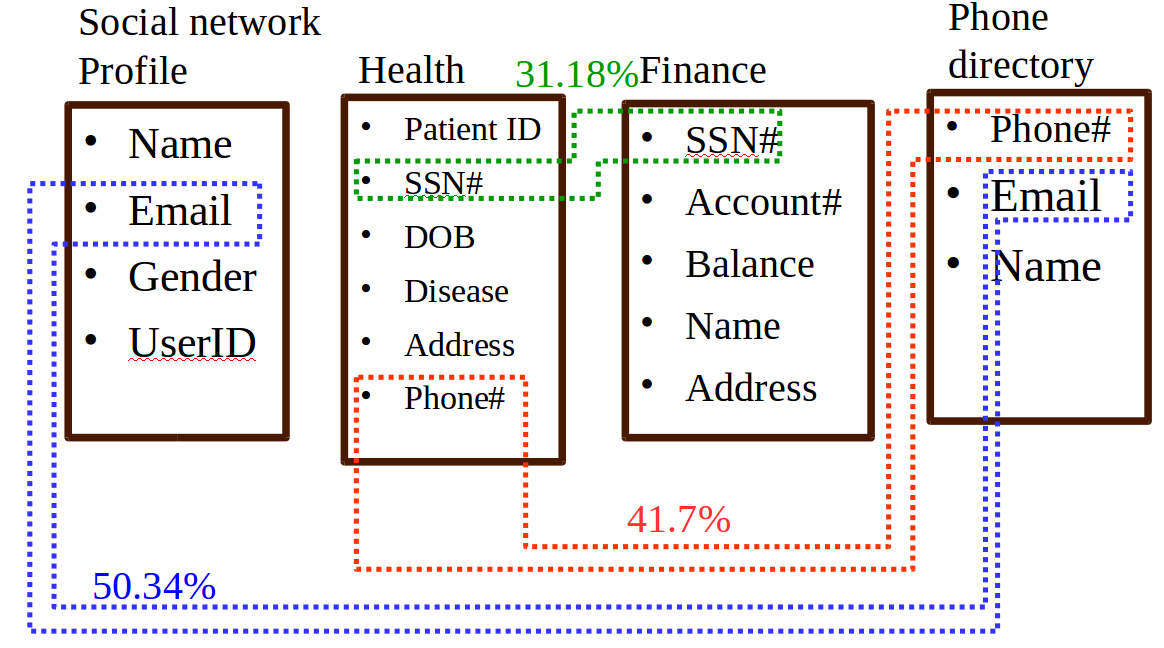
\includegraphics[width=0.7\linewidth]{figures/cross-correlationMap}
\caption[Cross-correlation map]{Four datasets containing $10^7$ documents with specific amount of cross-correlation are used in the estimation algorithm.}
\label{fig:cross-correlationMap}
\end{figure}

In order to attenuate the aforementioned problems, (computationally unfeasible  and inaccurate approximation), biased sampling method is considered to  provide more accurate responses for join aggregate queries. In such a scenario, extra information will be used for sampling from the base collections to preserve their relationships in the resulting sample set. The goal of this section is to use the extra information to produce biased sampling instead of random one. The class of documents with higher sensitivity ranking, the more possibility to be selected in the biased sample. In fact applying additional information (other attributes from the collection) in biased sampling phase facilitates cross-correlations discovering in the next phase. The biased sampling method only targets the highly sensitive attributes or the class of the interested documents selected from the database to form sample set. Although, biased sampling can be relatively pessimistic method, but since it focuses only on the crucial group of documents, the approximated answers are much closer to the exact answers. For example, consider two databases of secret devices and sensitive components, among which the correlation is supposed to be extracted. First, an AQP-based sensitivity analysis is performed on both collections to identify the most sensitive class in each database. Next, the biased samples are selected from these sensitive classes. The the proposed method has two phases, first, identifying correlated keys, second, approximating the size (cardinality) of cross-correlation using AQP approach.


\noindent \textbf{Correlated keys identification with AQP:} The idea is to first create a graph of documents using the biased samples. In the graph, there is an edge between vertex $i$ to vertex $j$ if they both have the same identifier attribute (such as phone number, social security number, patient ID, ... ). Finding connected components in an undirected graph which can be done with well-known graph search algorithms\footnote{Such as Depth First Search(DFS) or Breadth First Search (BFS) algorithms} starting from every unvisited vertex. Moreover, in the resulted graph the nodes with higher degree demonstrates attributes that cause more cross-correlation. The sorted list of vertices based on their degree exposes the attributes that cause more cross-correlation in pool of the cloud databases. The time complexity of this analysis is $O\big( \binom{m}{2}.n^2 \big)$, where $m$ is the number of samples and $n$ is the number of documents in each sample.

\noindent \textbf{ Cross-correlation analysis:} Analysis of information leakage, as a result of existence of \emph{unintentional cross-correlations} among many terabyte or petabyte level datasets, outsourced in the cloud DBaaS is a very hard problem with exponential growth rate. To overcome this problem, we adopt the approximation technique based on the correlated sampling to provide fast approximation with an acceptable error. This method is based on analyzing very small samples, and discovering potential relationships with other datasets. Consequently, a quick estimation of cross-correlation as clear indicator for information leakage will be achievable. The introduced approximation method eliminates the need for extensive analysis of the original datasets for cross-correlation discovery.

Consider two collections, $C_i, C_j$, let $\complement_{ij}$ be the exact cross-correlation between these collections. Cardinality of $\vert\complement_{ij}\vert$ presents the number of documents in $C_i$ and $C_j$ that have the same value for the correlation attribute. The subsequent subsections describe the cross-correlation size estimation method. 

%*************************************************
\subsection{Cross-correlation size estimation}
\label{correlatedEstimationSubSection}
%*************************************************

A set of random subset selected from the original collection which comprises of sensitive documents is constructed by uniform random sampling method. The selectivity probability $p_i$ for each sample $S_i$ is defined as $p_i=\frac{\vert S_i\vert}{\vert C_{i}\vert}$. In this method, first we apply AQP classification algorithm (discussed in the AQP classification section), to limit the cross-correlation analysis only to the much smaller space. In fact, with this approach, $\bowtie$ operator denoted as equality join is employed to measure the cardinality of cross-correlation between a uniform random sample $S_i$ joined to the biased sample. 

Suppose that, random sample sets are selected from users' profile database in a social media and phone directory which is limited to a particular demographic region of our interest. The average correlation size of those samples is a good approximation for true cardinality of correlation between the social media and phone directory. To deduce the estimated cross-correlation $\hat{\complement_{ij}}$,  Equation \ref{equ:CCEstimation} is used.

For instance, the average correlation size of random sample sets from users' profile database in a social media and phone directory which is limited to a particular demographic region is a good approximation for true cardinality of correlation between the that social media and phone directory. To deduce the estimated cross-correlation $\hat{\complement_{ij}}$ which is rephrased in Equation \ref{equ:CCEstimation}.

\begin{equation} 
\label{equ:CCEstimation}
\begin{aligned}
\vert \hat{\complement_{ij}}\vert=& \vert \complement^{\prime}_{ij}\vert \frac{1}{\min(p_i,p_j)}\\
\vert \hat{\complement_{ij}}\vert \approx & \vert \complement_{ij}\vert
\end{aligned}
\end{equation}
Where $\complement^{\prime}_{ij}$ is the cross-correlation between random sample $S_i$ and biased sample $S_j$ with selectivity probability of $p_i, p_j$ respectively.

%*************************************************
\subsection{Performance evaluation and experiments}
\label{PerformanceSubSection}
%*************************************************
We have a set of four datasets, including social network profile, health records, finance and phone directory each with $10^7$ documents. There are intentional cross-correlation between those datasets illustrated in Figure \ref{fig:cross-correlationMap}. The pipeline in the aggregate query is utilized to create equality join operator $\bowtie$ to extract documents from both given source and destination collections that match on the value of correlated attribute. The cross-correlation extractor query is displayed in Figure \ref{fig:CCQuery}. We applied the proposed estimation method to the sample sets with two different sizes and result is displayed in Figures \ref{fig:CCAproximation}. As it can be seen from figure, the bigger samples result in more accurate estimation. 

%Figure 
\begin{figure}[H]
\begin{framed}
{\ttfamily \small{ 
\textbf{db[source].aggregate}([\\\{\textbf{\$lookup :}\{\\\textbf{from :}destination,\\    \textbf{localField :}value,\\    \textbf{foreignField :}value,\\    \textbf{as :}"correlation" \}\},\\ \{\textbf{\$match :}\{"correlation":\{\textbf{\$ne :}[]\}\}\},\\
\{ \textbf{\$out :} saveToCollection \}\\]);
}
}
\end{framed}
\caption{Aggregate query for analysis of pairwise cross-correlation between two given source and destination collection.}
\label{fig:CCQuery}
\end{figure}


\begin{figure}[H]
\begin{subfigure}{0.5\textwidth}
\centering
\resizebox{1.0\textwidth}{!}{\begin{tikzpicture}[scale=1.0,trim axis right, trim axis right]
\begin{axis}[
compat=newest, 
legend style={at={(0.02,0.97)},anchor=north west},
ybar,
enlargelimits=0.12,
height=10cm,width=16cm,
bar width=20pt,
ylabel={Cross-correlation size},
symbolic x coords={{Health-Finance},{Social-Phone},{Phone-Health}},
xtick=data,
nodes near coords align={vertical}
,grid=major
,cycle list = {white,black!10,black!40,black!10,black!10}
]

\addplot+[fill=gray!80,text=black, draw=black, area legend,error bars/.cd,
y dir=both,y explicit] coordinates { %10000 documents
({Health-Finance},3123300)
({Phone-Health},5031080) 
({Social-Phone},4281100)
};
\addplot+[fill,text=black,  area legend,draw=black,pattern=north east lines,error bars/.cd, y dir=both,y explicit] coordinates { %100000 documents
({Health-Finance},3115910)
({Phone-Health},5036000) 
({Social-Phone},4265620)
};
\addplot+[fill,text=black, draw=black,  area legend,postaction={pattern=crosshatch},error bars/.cd, y dir=both,y explicit] coordinates { %Original correlation
({Health-Finance},3117847)
({Phone-Health},5033764) 
({Social-Phone},4170712)
};
\legend{Sample size $10^4$, Sample size $10^5$,Actual cross-correlations}
\end{axis}
\end{tikzpicture}
%\caption{}
%\label{fig:CCEstimation}}
\label{fig:CCEstimation}
\caption{}
\end{subfigure}
\qquad 
\begin{subfigure}{0.5\textwidth}
\resizebox{1.0\textwidth}{!}{\begin{tikzpicture}[scale=1.0,trim axis right, trim axis right]
\begin{axis}[
compat=newest, 
legend style={at={(0.02,0.97)},anchor=north west},
ybar,
enlargelimits=0.12,
height=10cm,width=16cm,
bar width=20pt,
ylabel={Error Percentage},
symbolic x coords={{Health-Finance},{Social-Phone},{Phone-Health}},
xtick=data,
nodes near coords align={vertical}
,grid=major
,cycle list = {white,black!10,black!40,black!10,black!10}
]
\addplot+[fill=gray!80,text=black, area legend, draw=black,error bars/.cd,
y dir=both,y explicit] coordinates { %10000 documents
({Health-Finance},0.6)
({Phone-Health},0.3) 
({Social-Phone},1.1)
};
\addplot+[fill,text=black,  area legend,draw=black,pattern=north east lines,error bars/.cd, y dir=both,y explicit] coordinates { %100000 documents
({Health-Finance},0.02)
({Phone-Health},0.02) 
({Social-Phone},0.95)
};
\legend{Sample size $10^4$, Sample size $10^5$}
\end{axis}
\end{tikzpicture}
}
\label{fig:speedup}
\caption{}
\end{subfigure}
\caption{The cardinality of cross-correlation estimation using two sets of samples with $10000$ and $100000$ documents: (a) Estimated values for the two sample sets, compared to the actual cross-correlation. (b) The estimation error percentage.}
\label{fig:CCAproximation}
\end{figure}
%*************************************************
\section{Conclusions and future work}
\label{sec:conclusion}
%*************************************************
For leakage prevention, insertion of disinformation documents is studied to break the links between the documents of among a group of datasets. Simultaneously, fake documents introduces two types of challenges to the systems. First, along with the data overhead growth, it causes system performance degradation. Second, the increase in communication cost between sever and the proxy which is due to transportation of the fakes documents.   

We introduced two techniques to mitigate the negative effects of data overhead. First, we present leakage quantitative methods to identify the leakage points in datasets; therefore, a selective disinformation document insertion is proposed to minimize leakage just in those points instead of the indiscriminate document insertion. Second, using multi-level indexes as one of the most efficient tools to improve query performance by maintaining unique values in a collection. With an index, the database process queries by simply scanning the index and fetching documents as they are refereed whereas without index entire table space must be searched. Thus the performance increase is substantial. 

We investigate explicit and implicit information leakage and practical metrics to evaluation and measurement are introduced. A fast sensitivity analysis method based on approximate query processing (AQP) for any dataset with multi-level sensitivity is presented. To enhance the performance and speed up of the AQP based classification we use multi-layer sampling with different sizes to provide query response with variety of acceptable error rates. Using AQP, elevates the scalability of sensitivity analysis to any database size in the interactive speed. With the proposed method, the large latency of analytical aggregate queries which severely limits the feasibility of many analysis applications will be resolved.

In addition, from both privacy and security perspective, having a limited access to the original database and instead processing the aggregate queries on very small set of samples is less risky for data owners in the cloud platform.

The process of AQP based classification using the uniform random samples provides adequate response with less computation and data access. In computer cloud, the proposed method demands fewer resources and much shorter computation time which contributes to less cost in cloud model. Ultimately, these features helps the cloud users to compute more complex aggregate computation through less expensive way.

Then, we propose a method to estimate the size of cross-correlation using biased sampling with reasonable level of inaccuracy. The optimum sample size results in subnational speed up in cross-correlation analysis with closer answer to the real value. Knowing all parameters including sensitive documents,attributes with high degree of connectivity and the cardinality of cross-correlation enables the data owners to selectively insert disinformation document only for sensitive attributes that contribute to high level of cross-correlations.

The sensitivity and cross-correlation analysis over multiple databases in cloud DbaaS only can be conducted with CSP who has access to all datasets. As future work, we suggest to have a cross-correlation monitoring service in public cloud. Form the privacy point of view it can be consider a users' privacy violation, but CSP might can define a Cross-correlation index (CCI) on small random samples of data and by using our method this index can be monitored  by CSP when its exceeds a specified amount, CSP alert the data owner. 

%*************************************************
\section*{Acknowledgment}
\label{sec:Acknowledgment}
%*************************************************
The authors wish to express their gratitude to an anonymous reviewer for constructive comments. We would like to extend our gratitude to Victor Shoup from New York University for NTL C++ library which is for manipulating arbitrary length integers.




%\appendix
\begin{appendices}
%*************************************************
\section{Leakage quantify algorithms} 
\label{app:Algorithms}
%*************************************************
\begin{algorithm}[H]
\caption{Construction of super document for an entity from multiple data collection}
\label{algo:ExractingLeakedInformation}
\begin{algorithmic}[1]
\Require{$S \subseteq W_{DBaaS},~\varepsilon$}
\Comment{$S$ is a set of collections, and $\varepsilon$ is an entity with document $d_i$}
\Procedure{SuperDocument}{$S$,$\varepsilon$}
\State  $L \gets \emptyset, ~\left\lvert \delta_{\varepsilon}\right\rvert \gets \{d_i\}$
\For{collection $D_j \in S$}
\For{document $d_k ~\in ~ D_j$}
\If{$(\mu(\delta_{\varepsilon},d_k)==TRUE)$}
\State $L_{\varepsilon} \gets \{New~arributes\}$
\State Update $\delta_{\varepsilon}$
\State Back Track
\Else \State continue
\EndIf
\EndFor
\EndFor
\State \textbf{return} $\delta_{\varepsilon}$ 
\Comment{Super document of entity $\varepsilon$}
\EndProcedure
\end{algorithmic}
\end{algorithm}


\begin{algorithm}[H]
\caption{Quantifying the mutual information of attributes from two data sources}
\label{algo:mutualInformation}
\begin{algorithmic}[1]
\begin{varwidth}[t]{\linewidth}
\Require{$S,~T$ : Source and Target data vector, $n$ Length of vector non-empty $n > 1$}
%\item[]
\Procedure{MutualInformation}{$S$,$T$,$n$}
%\Comment{$I(X;Y) = \sum p(xy) * \log (p(xy)/p(x)p(y))$} 
\State $sProbs \gets calculateProbility(S,n)$  
\Comment{Probability vector of $S$}
\State $tProbs \gets calculateProbility(T,n)$ 
\Comment{Probability vector of $T$}
\State $MutualInformation \gets 0.0 $
\State $jointProbVector= calculateJointProbability(sProbs,tProbs,n)$

\For{$(i \in n^2 )$}
\State $firstIndex=i\mod n$
\State $secondIndex=i /n$
\If{$((jointProbVector[i]>0)$\par
\hskip\algorithmicindent $\&~(sProbs[firstIndex]>0)$\par
\hskip\algorithmicindent $ \&~(tProbs[secondIndex]>0))$\par
\hskip\algorithmicindent }
\State $mutualInformation\bm{+=}$\par
\hskip\algorithmicindent $jointProbVector[i] \bm{ \times}\log(jointProbVector[i] \bm{/}$\par \hskip\algorithmicindent $(sProbs[firstIndex] \bm{\times} tProbs[secondIndex]))$
\EndIf
\EndFor
\State   $mutualInformation \bm{/=} \log(2.0)$
\State \textbf{return} $mutualInformation$
\EndProcedure
\end{varwidth}
\end{algorithmic}
\end{algorithm}
\medskip


\begin{algorithm}[H]
\caption{Selective disinformation insertion algorithm}
\label{algo:disnformation}
\begin{algorithmic}[1]
\Require{$D$}
\Comment{Original dataset}
\Require{$\mathcal{V}$}
\Comment{Rate of disinformation to information}
\Require{$T$}
\Comment{Acceptable level of leakage}
\Ensure $\widetilde{D}$
\Comment{Data set diluted with disinformation documents}
\item[]
\Procedure{diluteDatabase}{$D, \mathcal{V}, T$}
\State $\Psi \gets evaluateLeakage(D)$
\Comment{Statistical analysis}
\State $\tau \gets \mathcal{V}$
\For{\textbf{each} (pair $d_i,d_j$ in $D$)}
\If{$(\Psi.L(d_i,d_j)> T)$}
\While {$(\tau)$}
\State $\rho \gets\ createDisInformation(d_i,d_j)$
\Comment {New disinformation document $\rho$ is created.}
\State $insertToDatabase(D, \rho)$
\State $\tau \gets \tau-1$
\EndWhile
\EndIf
\EndFor
\State \textbf{return} $D$ 
\Comment{Diluted dataset}
\EndProcedure
\end{algorithmic}
\end{algorithm}
\medskip
%*************************************************
\section{Metric for explicit information leakage}
\label{app:primaryMetric}
%*************************************************

We define a notion to show what portion of disinformation is valid, by adapting {\it precision}, {\it recall} and {\it F-Measure} from information retrieval and binary classification literature \cite{davis2006relationship}. In general, precision\footnote{Indicates how many relevant items are selected }, recall\footnote{Indicates how many selected items are relevant} and F-Measure\footnote{ Harmonic mean of precision and recall} are simple metrics for quantifying valid information found inside any given document. The precision takes all attributes of document $d$ into account fo find the number of those attributes which are member of the super-document of attributes. The higher precision value means more common attributes that increases the probability of being merged into the super-document provided that at least of the attributes is from identifier class or group of them are semi-identifier. In this case, the uncommon attributes are considered as leaked information. The recall measures the strength of merge capability of a pair of documents (see Equation \ref{eq:leakageMetrics}). Precision of document $d$ denoted as $P_d$ which is a fraction of information in document $d$ with respect to super-document  $\delta$ containing attributes that their authenticity is established. \textit{Recall} and \textit{F-Measure} for document $d$ are denoted as $R_d$ and $F_{1}$ respectively:
\begin{equation} 
\label{eq:leakageMetrics}
\begin{aligned}
P_d=\frac{\left\lvert d \cap \delta \right\rvert}{\left\lvert d \right\rvert},\qquad 
R_d=\frac{\left\lvert d \cap \delta \right\rvert}{\left\lvert \delta \right\rvert},\qquad
F_{1}=\frac{2 \times P_d \times R_d}{P_d + R_d}
\end{aligned}
\end{equation}

The concepts of precision and recall based on document and super-document are demonstrated in more detail with an example. By definition, the super-documents includes all the accurate attributes ($A_i$) related to an object of interest. The document, on the other hand, includes inaccurate and/or fake attributes ($\mathcal{F}_j$). The fake documents are actually the noisy documents (disinformation) which is added to the collection in order to minimize the information leakage. A small fraction of document includes accurate attributes and the remaining are false. If the common attributes between the document and super-document are minimized, the lower information leakage is warranted. Consider Figure \ref{fig:PrecisionRecall} in which super-document $\delta$, includes $8$ accurate attributes and document $\delta$ includes $5$ (i.e. $2$ accurate and $3$ fake) attributes.\\

%Figure in the tex file
\begin{figure}[h]
\centering
\begin{tikzpicture}
\node[box2, fill=white, fill opacity=0.2] (c2) at (0,0) {};
\node[box2, fill=gray!20, fill opacity=0.3] (c1) at (4.5,0) {};
\fill[blue!20,fill opacity=0.2] (2.25,0) circle (2cm);
\draw (2.25,0) circle (2cm) node [above] {};
\node[label={\large Relevant Attributes}]  at (-0.15,2.2) {};
\node[label={\large Irrelevant Attributes}]  at (4.5,2.2) {};

\fill[black] (-1.5,1.0) circle (0.25cm);
\node[label={\small $A_6$}]  at (-1.5,1.0) {};

\fill[black] (0,1.0) circle (0.25cm);
\node[label={\small $A_2$}]  at (0,1.0) {};

\fill[black] (1,0.5) circle (0.25cm);
\node[label={\small $A_3$}]  at (1,0.5) {};

\fill[black!50] (3,1.0) circle (0.25cm);
\node[label={\small $\mathcal{F}_1$}]  at (3,1.0) {};

\fill[black!50] (5.5,1.0) circle (0.25cm);
\node[label={\small $\mathcal{F}_4$}]  at (5.5,1.0) {};

\fill[black] (-1.5,0.0) circle (0.25cm);
\node[label={\small $A_4$}]  at (-1.5,0.0) {};

\fill[black] (-0.4,0) circle (0.25cm);
\node[label={\small $A_5$}]  at (-0.4,0.0) {};

\fill[black!50] (3.7,0.0) circle (0.25cm);
\node[label={\small $\mathcal{F}_2$}]  at (3.7,0.0) {};

\fill[black!50] (5,0.0) circle (0.25cm);
\node[label={\small $\mathcal{F}_5$}]  at (5,0.0) {};

\fill[black] (-1.5,-1) circle (0.25cm);
\node[label={\small $A_8$}]  at (-1.5,-1) {};

\fill[black] (0,-1) circle (0.25cm);
\node[label={\small $A_7$}]  at (0,-1) {};

\fill[black] (1,-1) circle (0.25cm);
\node[label={\small $A_1$}]  at (1,-1) {};

\fill[black!50] (3.0,-1) circle (0.25cm);
\node[label={\small $\mathcal{F}_3$}]  at (3.0,-1) {};

\fill[black!50] (5.5,-1) circle (0.25cm);
\node[label={\small $\mathcal{F}_6$}]  at (5.5,-1) {};

\end{tikzpicture}
\caption{An example to demonstrate Precision and Recall}
\label{fig:PrecisionRecall}
\end{figure}

\begin{align*}
\delta&=\{A_1,~A_2,~A_3,...,~A_8\}\\
\rho&=\{A_1,~A_3,~\mathcal{F}_1,~\mathcal{F}_2,~\mathcal{F}_3\}\\
\rho \cap \delta &=A_1,~A_3; \qquad \left\lvert \rho \cap \delta \right\rvert=2\\
P_{\rho}&=\frac{\left\lvert \rho \cap \delta \right\rvert}{\left\lvert \rho \right\rvert} = \frac{2}{5},\qquad 
R_{\rho}=\frac{\left\lvert \rho \cap \delta \right\rvert}{\left\lvert \delta \right\rvert}= \frac{2}{8},\qquad
F_{1}=\frac{2 \times P_{\rho} \times R_{\rho}}{P_\rho + R_\rho}= \frac{0.2}{0.65}=0.307
\end{align*}

%*************************************************
\section{Metric for implicit information leakage} 
\label{app:infoTheoritic}
%*************************************************
Given any two data fields which can be represented by two random variables $X,Y$, their values are chosen from two value sets $\chi, \gamma$ respectively. The probability distribution of these two random variables can be expressed with $p\left( x \right)=P \left[ X=x_i\right]$ and $p\left( y \right)=P\left[Y=y_j\right]$. 

\begin{equation}
\label{equ:Leakagedefinition}
\begin{aligned}
\noalign{\text{Value sets $\chi$ and $\gamma$ are defined as:}}\\
&\chi=\{x_1,\ldots,x_n\}, ~ \gamma=\{y_1,\ldots,y_m\}\\
&\text{Where $X,Y$ chosen values are from value sets $\chi, \gamma$ such that:}\\
&X: \chi \longmapsto x_i ~and~  Y:\gamma \longmapsto y_j\\
&\text{Knowing that the {\it entropy} of $X,Y$ are defined as:} \\
&H(X) = -\sum_{i=1}^{n}p(x_i) \log p(x_i); \quad
H(Y) = -\sum_{j=1}^{m}p(y_j) \log p(y_j)\\
\end{aligned}
\end{equation}

The {\it conditional entropy} that measures the uncertainty of $X$ when $Y$ is known is defined as below: 

\begin{equation}
\begin{aligned}
& H(X|Y) = -\sum_{i,j} p(x_i,y_j) \log \frac{p(x_i,y_j)}{p(y_j)} \quad =  \sum_j p(y_j) H(X|Y=y_j)\\
& \text{A chain rule for multiple random variables holds:}\\
& H(X_1,X_2,\ldots,X_k) = \sum_{i=1}^k H(X_i | X_1, \ldots, X_{k-1}) 
\end{aligned}
\end{equation}
If the random variables $X,~Y$ are independent, the value of $\mathcal{L}(X,Y)$ is $0$. The value of $\mathcal{L}(X,Y)$ is maximum if $X,~Y$ are completely dependent. Therefore, the {\it information leakage} between two data elements $X,Y$ is presented as $\mathcal{L} \left(X,Y\right)=H\left(X\right)-H\left(X \lvert Y\right)$. In other word, $\mathcal{L}(X,Y)$ measures the information that can be captured about $X$ provided that we know $Y$. $\mathcal{L}(X,Y)$ is commutative relation and its value is a number in the range of $0$ and $H\left(X\right)$. 
\begin{equation} 
\label{eq:leakage}
\mathcal{L} \left(X,Y\right)= \mathcal{L}\left(Y, X\right)= 
\begin{cases}
0   & \quad \textbf{if}  ~ X,~ Y ~~~~~ \text{ are independent}\\
H\left(X\right) & \textbf{When}  ~ X,~ Y~~   \text{ are completely dependent}
\end{cases}
\end{equation} 

\noindent {\bf Mutual information of attributes:} We define {\it mutual information } for quantifying the relationship between two attributes belonging to any two selected databases. In particular, it measures how much information is found in one attribute about another and vice versa. An important theorem from information theory states that the mutual information between two variables is 0 if and only if the two variables are statistically independent. The formal definition of the mutual information of two random variables $X$ and $Y$ , $I(X; Y)$, is given by: 

\begin{equation} 
I(X; Y ) = \sum_{i}\sum_{j} P\left(x_i, y_j\right) log \left(\frac{P\left(x_i, y_j\right)}{P\left(x_i\right)P\left(y_j\right)}\right).
\end{equation} 
In this definition, $P\left(x_i\right)$ and $P\left(y_j \right)$ are the marginal distributions of $X$ and $Y$, and $P\left(x_i, y_j \right)$ is joint probability of $X, Y$. Mutual information evaluates  the binary relation that indicates the information that $X$ and $Y$ are shearing. In particular, it measures how much knowing one of these variables reduces our uncertainty about the other. Intuitively, mutual information can be interpreted as a definition of information leakage.\\

In general, information leakage between multiple data elements can be define using conditional mutual information, a form of multi-tier interaction. Particularly, conditional mutual information measures the correlation between two random variables conditioned on a third random variable an so on; it is defined as:
\begin{equation} 
I(X; Y|Z) = H(X|Z)-H(x|Y,Z)= H(Y|Z) - H(Y|Y,Z)
\end{equation} 
\end{appendices}

 %	BIBLIOGRAPHY
\bibliographystyle{IEEEtran}
\bibliography{reference}
 %----------------------------------------------------------------------------------------
 \end{document}
